
\begin{savequote}[8cm]

    We hear a lot these days about genes and molecules, but how does one human brain, or one human being coordinate, or entrain, or resonate with another?  We may not realise it but we live in a world of coordination, at every level and every scale of endeavour.

  \qauthor{--- J. A. S. Kelso  \textit{Coordination and the Complimentary Nature} Presentation to the The New York Academy of Sciences - May 12, 2010}
\end{savequote}


%I do not see any way to avoid the problem of coordination and still understand the physical basis of life.
%\qauthor{--- H. H. Pattee  \textit{The role of instabilities in the evolution of control hierarchies} 1976}


\chapter{\label{theory}A theory of social bonding through joint action}


\minitoc

\section{Abstract}

In this chapter I outline a novel theory of social bonding through joint action, which will be tested in subsequent empirical studies of Chinese rugby players.  In particular, I identify team click as a special case phenomenon of joint action and a potential mediator of the relationship between joint action and social bonding in group exercise contexts.  Emerging research from the social cognition of joint action suggests that a continuum of cognitive mechanisms are responsible for establishing and maintaining complex and intricate behavioural coordination between two or more individuals.  I consider the role of inter-individual and cultural variation in knowledge, expertise, experience, and personality type in modulating these mechanisms. I conclude the chapter by summarising a theory of social bonding through joint action, and outlining predictions that arise from this theory.







                                            \begin{CJK}{UTF8}{gbsn}

\section{Vignette: Sun Hongwei, Beijing's newest recruit}}
Sun Hongwei arrived, escorted by his high school athletics coach, to the Beijing Temple of God of Agriculture Institute of Sport (hereafter the Institute) soon after I began my fieldwork in August 2015.  An 18-year-old with a slight build and timid demeanour---his gaze remained diverted to the ground during his first few months at the Institute---Hongwei had never seen a rugby ball before that day he arrived.

Hongwei was from Hebei province, immediately surrounding the special prefecture of Beijing, China's capital.  As was relatively common practice at the time in the Chinese competitive sport system, Hongwei's coach had organised a trial for Hongwei with the Beijing Provincial Men’s and Women's Rugby Program (hereafter the Rugby Program) by calling upon social connections to the leadership of the Institute.

Athletes come to the Rugby Program from all over the country.  Representing Beijing at a provincial level in a sport like rugby can translate into the opportunity to gain entrance---via a designated ``specialist athlete'' (\textit{tiyu techan} 体育特产) pathway---to one of China's top universities (Beijing Sports University, in this case) and enhanced career employment opportunities thereafter.  Rugby is not a popular sport in China. It is referred to as a neglected branch of the Chinese sport system, or a ``cold-gate'' (\textit{lengmen xiangmu} 冷门项目), referring to a profession, trade or branch of learning that receives little attention). Despite its minnow status in China in terms of its popularity, rugby's recent inclusion in the Olympics (in the form of the modified seven-a-side version of ``rugby sevens'') means that it now occupies a prominent place in the Chinese sport system, which has been defined since its inception by a strong Olympic logic \citep{Brownell2008}.  If a sport is a current member of the summer or winter Olympic Games, then the sport is included in the roster of sports played at the quadrennial China National Games (\textit{quanhunhui}). As such, rugby programs such as the one at the Institute now exist in twelve of China's 34 provincial level regions, either embedded within, or somehow associated with, tertiary education institutions.  Thus, although rugby and China are two words that have not historically featured within the same utterance, rugby in China now affords athletes a rare and under-capitalised opportunity to pursue attractive life-course opportunities of education and employment in an intensely competitive education system.

Without exception, the athletes who arrive at the Institute to join the rugby team have not spent their childhoods playing rugby in their schoolyards or watching professional rugby on television. Many who come to rugby transition from other more popular sports such as athletics, basketball, or association football, and often---like Hongwei---have never seen a rugby ball before they arrive.  Most ``start from scratch,'' so to speak, in terms of their grasp of the requirements of the highly interactive and technically complex team sport. In addition to complex patterns of movement coordination, rugby also involves unrestrained body-on-body collisions and intense bouts of high physiological exertion, requiring speed, strength, agility, and endurance to perform all of rugby's technical requirements successfully.  Learning the game of rugby from a baseline of essentially zero, while also navigating the inevitably demanding  social and political dynamics within the team and the Institute, was clearly going to be a daunting task for Hongwei.

                        \begin{center}
                          * * *
                        \end{center}

Hongwei was the first of the Program’s new recruits that I followed closely.  Even compared to other newly arrived junior athletes, he was noticeably timid and shy, particularly in his interactions with the coaches (myself included) and senior players. Nevertheless, Hongwei clearly signalled diligence and commitment through his participation in team activities, arriving early to each training session, and carrying more than his fair share of the training equipment---a task shared by the most junior members of the team.  Each time I passed Hongwei in the corridors of the Institute he would greet me with a polite bow and greeting, ``Hello Coach'' (\textit{'jiaolian hao'} `教练好').  In these instances, Hongwei would coordinate his greeting with a moment's eye contact, only to return his gaze to the floor and continue walking.

Due to his initial lack of familiarity with the basic techniques of rugby, Hongwei was unable to properly participate in normal training with the rest of the team.  Instead, during the first month or so, Hongwei stood on the sidelines and practiced the basics with other athletes who were unable to fully participate in training due to injury: learning how to pass and catch the rugby ball, both stationary and in-motion. In my eyes at least---those of an observer accustomed to instinctual grasp of these movements from a young age---Hongwei's attempts to accustom himself with the skills of rugby were jarring.  The idiosyncrasies of rugby's bizarrely shaped ovular ball often foiled Hongwei. I would regularly see him chasing after a ball on the ground he'd just fumbled, as if he was chasing in vein after a scurrying rabbit tactfully evading his pursuit.

Whilst coaching and playing rugby in China, I watched many start exactly as did Hongwei: on the sidelines of training, learning how to pass the ball.  But for some reason I found Hongwei’s attempts to learn particularly unusual.  His actions appeared so mechanical that it was almost as if he was deliberately (over)imitating the required actions of passing, catching, and running as an overt signal of diligence and commitment.
%---> I will work on re-wording this

A few weeks into Hongwei’s time at the Institute, I asked head coach Zhu Peihou about his newest recruit.  He immediately shook his head and scrunched up his face dismissively, adding in a disappointing whisper, ``no good'' (\textit{buxing} 不行).  Chinese rugby coaches are well acquainted with athletes starting from scratch with the technical requirements of rugby---they were used to things looking awkward and ugly at the start.  Coaches are usually more interested in the physical raw materials that enable athletes to develop into rugby players over time.  Often this means that coaches have a habit of fixating on an athlete's baseline characteristics (e.g. height and body frame) as an indication of his or her capacity to develop the physical speed, size and strength deemed crucial for elite performance.  Also important, but less crucial than physical attributes, are an athlete’s baseline ball-handling skills and ``game sense'' (\textit{qiugan} 球感)(which coaches often assess by observing new recruits participating in analogous interactive team sports, like basketball or association football).

Hongwei was still relatively young and physically undeveloped when he arrived, but it was already clear that he was not endowed with a big physical frame; nor was he noticeably fast or agile compared to other athletes.  For these reasons, I assumed, head coach Peihou couldn’t help but let on to me that he was not particularly excited about Hongwei's future prospects in the Program.  In fact, I got the sense that Peihou's reaction to my question contained an element of annoyance or frustration with the terms under which Hongwei had arrived to the Institute, i.e., via the arrangements of Hongwei’s athletics coach.  According to Zhu's own assessment of Hongwei's ability and future potential, the head coach was perhaps conceding to me that he had been forced to accept an athletic dud into the team.

                        \begin{center}
                          * * *
                        \end{center}

I first interviewed Hongwei approximately six weeks after he arrived at the Institute.   Hongwei's demeanour during the interview was consistent with the timid and shy one that he presented publicly at training.  As explain below, he did show some signs of captivation with his new sport and social environment.  When I asked about his initial impressions of the on-field demands of rugby, however, Hongwei was quick to confess that he felt utterly unacquainted:

\begin{quotation}
  SHW: I still haven’t really started to practice any of the team plays or anything; all I can do so far is pass and run a little bit...(but) it's quite fun! \\
  JT: What do you think is the most difficult component of rugby? \\
  SHW: Um\textellipsis well, coordinating with teammates [on the field], particularly coordination in attack.  Because I can't figure it out.  When I first arrived, I didn’t even know what a ``switch play'' or a ``blocker play'' was.
\end{quotation}

  \begin{quotation}
    SHW: 战术没怎么接触,就是像传球啊、跑动什么的会一点了 \\
    JT: 感觉怎么样?\\
    SHW: 挺好玩的!\\
    JT: 你认为橄榄球最难的一部分是什么? \\
    SHW: ...打配合,进攻的配合,因为搞不明白,刚来的时候也不知道什么交叉,后插什么的 \\
  \end{quotation}

Hongwei was self-critical in his confession regarding his minimal grasp of the technical requirements of joint action in rugby. His confession was indicative of a broader trend with the other athletes I interviewed, as I will explain in more detail in the ethnographic sections of this dissertation (see Chapters ~\ref{4partAIntroMethod}\nobreakdash~\ref{6ethnographicResults}). When athletes were asked in interviews about the most difficult aspect of rugby, on-field coordination with teammates was by far the most common answer, particularly among the new recruits and most junior athletes.

As I directed the interview towards topics beyond the on-field technical demands of rugby, Hongwei was more positive, framing rugby as an exciting new opportunity, and commenting that his friends and family were in awe of the fact that he is playing such an impressively ``strong'' physical sport like rugby.  When I asked him about something new that he had learnt through playing rugby, Hongwei automatically responded by emphasising the social dimensions of his experience at the Institute:

\begin{quotation}
  ``...I think it's mainly this thing of having teammates. Before, when I was training for an individual sport, it was just me training by myself. [In that environment] it was a case of whoever trained well was successful.  But now with this team of brothers, elder teammates will take care of younger teammates. We all train together, and if you can’t do something, you can always ask your elder teammates...[Rugby] is so much better, because in an individual sport, if you can't master something, you have to go to your coach for help. Other athletes don't want to teach you, because if you surpass other people, then they have to work even harder to keep up... I have had to learn about helping each other, because rugby is not like an individual sport, where you look after your own performance and that's it.  In a team sport, if you don't do well, there's no need to get too frustrated or upset, because other athletes will help you out, and I will also help others out, that type of collaboration with each other.''
\end{quotation}

\begin{CJK}{UTF8}{gbsn}
  \begin{quotation}
    我觉得主要是师哥师弟的这一块儿,原来练个体项目都是自己练自己的,谁练好了谁厉害,但是现在师哥师弟,有师哥照顾师弟带着,互相练,我不会我可以问师哥
    ...因为个人项目你不会就必须要找教练,但是别人不愿意教你,因为你把别人超越了那别人还还得努力。 学到互相帮助,因为向个体项目自己成绩自己来拿就行,而像团体项目,即使自己做不好,也不用太泄气太沮丧,因为别人会帮你做好,我也会帮别人做好,互相协作的那种.
  \end{quotation}
\end{CJK}

Through his explicit reference to the fraternity of the team, and his position as junior member, Hongwei highlights that the technical skills of rugby were not the only important novelties.  Hongwei's background was as a pentathlete (track and field / athletics---an individual sport), and the team environment was completely new to him, as it was to many other athletes in the team.  As I listened to his experiences associating rugby and group membership, I could not help but associate the quality of these declarations of prosociality with his overly mechanical imitation of rugby's foundational techniques.  It was as if both were equivalently diligent (albeit somewhat awkward and un-habituated) signals of team commitment.

                              \begin{center}
                                * * *
                              \end{center}

A few months passed, and Hongwei continued to train.  He was as eager and committed as when he began, and I did notice some gradual improvement in his grasp of rugby's basic skills.  But he also remained extremely reserved, keeping his head low at all times in team settings, unless addressed by senior players or coaches.  Then, one evening when I had returned to my room in the Institute dormitory from a three-week hiatus in Australia over Christmas of 2015, I heard a knock on my open door, and to my surprise Hongwei took an assertive stride into my room, carrying in two arms a draw-string bag containing rugby balls (which were in need of more air before the next day's training session).  Hongwei had never ventured into my room before, apart from our first interview two months earlier, but never on his own accord.  Remarkably, Hongwei looked me straight in the eyes with his head held high and energy beaming from his face and chest.  I couldn't help but smile and ask, with genuine intrigue, ``How has training been recently?''
``Very good'' he said, assertively and excitedly.  ``Much better than before.  At least now I know what’s going on at training, I can keep up with the plays!''  A big smile grew on his face as he continued to hold my gaze.  ``Oh good!'' I said. I congratulated him for his hard work in training while I had been away, and encouraged him to keep at it.  Wow, I remember thinking to myself, Hongwei was possessed by a powerful force.  Somehow, Hongwei, rugby, and the team in which he was by now more comfortably enmeshed had clicked into place to instil him with a visceral sense of agency.
%(I felt like giving him a pat on the back and suggesting that he try to relax and take the weight off his shoulders, thinking that his anxiety about fitting in may be getting in the way of the ultimate goal of fast-tracking skill acquisition!)
%Hongwei had begun to develop an innate feel for the game.

                          \begin{center}
                            * * *
                          \end{center}


\subsection{Vignette 4}
A few weeks later, head coach Wang (who took over from Peihou, who abruptly resigned while I was away in Australia), told me that he had decided to take Hongwei to pre-season training in Guangzhou, for a month starting in March 2016.  Chongyi admitted that while Hongwei was perhaps not the most promising of the junior athletes, his attitude was very good:

  \begin{quotation}
He [Hongwei] likes to train, and he is very diligent. I want to take his positivity with us [to Guangzhou] \\
他爱练,而且很用心,带上他的积极性过去
  \end{quotation}


                          \begin{center}
                            * * *
                          \end{center}


These ethnographic observations relating to Hongwei's first four months at the Institute highlight key themes of this dissertation.  As I discuss in more detail in this chapter, existing research suggests that successful coordination in joint action requires alignment and maintenance of equivalent expectations between co-actors \citep{Sebanz2006,Vesper2017,Pesquita2017}.  Importantly, evidence also suggests that violation of expectations in joint action has strong affective consequences \citep{Chetverikov2016}.  The fact that Hongwei's familiarity with the technical requirements of rugby appeared over time to co-vary with aspects of his personal demeanour suggests a relationship worthy of further investigation.  As I explore in Chapters LINK and LINK, my ethnographic observations reveal broader patterns of within-group variation between perceptions of joint action performance, team click, and social bonding.  These observations, coupled with predictions from existing literature within the social cognition of joint action, set the foundations for subsequent field-experimental studies in which I test specific relationships with a broader subset of Chinese professional rugby players beyond the Beijing Men's Team.

How is it possible to scientifically account for the unmistakably ``visceral'' quality of Hongwei's transformation from timid newcomer to budding Beijing rugby player?  How can these ethnographic observations be explained in terms of generalisable cognitive mechanisms and systems dynamics of joint action?  Finally, and ultimately, how do answers to these questions improve our ability to comprehend the evolutionary significance of group exercise in the human record?


HW's change is a change in attitude (Bateson)
agency










\section{Introduction}
The human capacity to coordinate behaviour within cohesive social groups is a fundamental explanation for our species' evolutionary success \citep{Tomasello2009}.  It is surprising that sport---an ubiquitous organiser of modern social life and physical movement across cultures---has not been more intensively studied for evidence concerning the cognitive and social foundations of human evolution \citep{Blanchard1995,Downey2005a}.  An integrated scientific study of the physiological and cognitive mechanisms and ecological dynamics associated with coordination of movement stands to offer novel insights into the phenomenon of group exercise.  In this dissertation I attend specifically to the relationship between joint action and social bonding in the group exercise context of professional rugby in China.  In this chapter I formulate a novel theory of social bonding through joint action in order to address the knowledge gaps in the social high theory of group exercise and social bonding.

Physical movement is central to the adaptive success of biological life, particularly life for which movement can intentionally directed in order to bring about change in the environment.  The ability of humans to cooperate with one another vastly increases the range of their potential actions \citep{Clark1996}.  Humans display a rich capacity for complex forms of autonomic and preconceived physical movement, which is employed both when coordinating behaviours with the environment and socially with conspecifics.  The ultra-social nature of the human species dictates that all human movement has a latent action potential---everything from ostensive communicative signals to implicit cues derived from inadvertent movement can carry a social charge \citep{Danchin2004}, and it appears that humans have evolved reward mechanisms for adaptive coordination of movement with conspecifics and the physical environment \citep{Wheatley2012,Parkinson2015,Wheatley2016}. Within cognitive science and psychology, the term \textit{action} is used to distinguish intentional, agent-directed movement from other forms of movement \citep{Davidson1980}.  Specifically, the term ``joint action'' can be used to describe any form of social interaction whereby two or more individuals coordinate their actions in space and time to bring about a change in the environment \citep{Sebanz2006a}.

\subsection{Joint action beyond synchrony}
As discussed in the previous chapter, experimental evidence from the behavioural synchrony and mimicry literatures suggests that exact synchronisation of movement between co-actors in joint action may be a powerful generator of trust and affiliation between co-actors in joint action.  Synchrony appears to be responsible for positive affect, blurring of self-other agency, spontaneous pro-social behaviour, and reinforcement of cooperation \citep{Mogan2017}, and these effects could be underwritten by the activation of neurobiological reward systems \citep{}.  This evidence leads to the suggestion that the effects of behavioural synchrony, in addition to those of physiological exertion, combine in group exercise contexts to generate a psychophysiological environment conducive to forging social bonds \citep{Cohen2017}.

Synchronisation is defined as a process in which two independent components continuously influence each other toward greater entrainment (within a certain lag tolerance) such that synchronising parties reduce overall variance of their joint activity, making them more similar and more regular \citep{Pikovsky2007}.  For the social high theory of group exercise (outlined in Chapter ~\ref{introduction}), behavioural synchrony an obvious place to begin.  Synchrony is a highly ordered form of phase- and frequency-locked coordination, which is relatively easy to operationalise in experimental settings with naive participants, and which provides a clear demonstration of motor and cognitive entrainment between individuals.  Care should be taken in not becoming overly fixated on behavioural synchrony as an ideal expression of coordination in group exercise contexts, for at least two reasons.

\subsubsection{Detailed components of Joint action}
First, while Synchrony is a fast and efficient way in which to achieve motor and cognitive entrainment between two or more individuals, using synchrony as an experimental stand-in for for interpersonal coordination in joint action simplifies joint action and occludes its various component mechanisms.  In real world situations, coordination in joint action involves temporal and spatial precision and flexibility of interpersonal movement regulation across multiple timescales and sensorial modalities in order to bring about change in the environment \citep{Sebanz2006}. Joint action demands a suite of realtime coordination skills.  In order to successfully entrain with others in joint action, participants must constantly anticipate, attend, and adapt to the actions of others and the circumstances of the task-specific environment \citep{Keller2014}. Participants rehearse task-specific skills individually and together over extended periods of time to produce a hierarchy of aligned representations that form the basis of an implicit common ground for successful joint action \citep{Noy2017}.  These skills are constrained by shared knowledge of the task environment \citep{Vesper2017} and modulated by individual differences in personality type and social orientation \citep{Marsh2009,Keller2014}.

When performing joint action, people move in a more predictable way than when moving alone \citep{Vesper2011}, and demonstrate an ability to be more or less cooperative by altering the level of compensatory temporal and phase correction in response to partner's actions \citep{Repp2008}.  These tendencies give rise to a range of entrainment patterns in joint action, such as a leader-follow dynamic \citep[usually in situations where there is a skill disparity between participants,][]{Fairhurst2014}, or a mutually synchronised ``co-confident'' entrainment, which lacks the typical jitter resulting from the reactive control of a leader-follower dynamic \citep{Noy2011,Noy2015}.  Participants often deviate from planned movement (either intentionally or unintentionally), according to familiarity, technical competence, or past experience with the specific joint task \citep{Goebl2009}.  In sum, when coordination is operationalised as strict synchrony, many crucial component mechanisms that precede successful entrainment and social bonding are occluded from view and are potentially overlooked as candidates for explaining a relationship between joint action and social bonding.


\subsubsection{Synchrony as a special case in functional synergies}
Second, a fixation on synchrony alone can lead to the misleading prediction that optimal coordination in joint action should resemble progress toward similarity and equivalence of action between co-actors \citep{Fusaroli2014}.  Strict in-phase behavioural synchrony, although immediately eye-catching and identifiable in well-known group activities such as group dancing, military drills, or sports like rowing, is in fact atypical of most instances of interpersonal coordination.  The corpus of human interpersonal coordination reveals instead that coordination in joint action is more often achieved through function-specific assemblages of complimentary and contrasting behaviours (for example, a dyadic conversation or an ensemble music performance).  Dynamical systems approaches to behaviour and cognition demonstrate that movement coordination involves processes that are in constant flux and subject to self-organising dynamics typical of multi-element systems \citep{Turvey1977}. As such, coordination processes should be modelled as ``functional synergies'' (SOURCE).  Functional synergy offers a unifying model for different levels of analysis from brain \citep{Yufik2013} and motor coordination \citep{Latash2007}, to perception-action coupling \citep{Kelso2009} and to interpersonal coordination in joint action \citep{Riley2011,Schmidt1990}, and even cultural evolution \citep{Claidiere2007a}.  From a ``coordination-as-functional-synergy'' perspective, synchronisation in joint action is only one special case, rather than coordination's inevitable or ideal end-state \citep[128][, Richardson, personal communication]{Kelso2013}.  The relationship between states of coordination in joint action beyond exact in-phase synchrony and social bonding is yet to be thoroughly explored \citep[but for a preliminary approach, see][]{Marsh2009}.


\subsubsection{Overview of a novel theory of social bonding through joint action}



%Anecdotal and observational evidence from anthropology and psychology---particularly the psychology of ``flow'' \citep{Csikszentmihalyi1992,Jackson1999}---suggests that perceptions of joint action success may set the psychological foundation for processes of affiliation.  Various neurological, cognitive, and sociological strands of evidence support this proposal.  Perceptions of successful coordination of behaviour in joint action appears to have positive implications for individual psychophysiological function, health, and subjective well being \citep{Wheatley2012}.  Likewise, there is well-documented evidence of a link between psycho-social isolation and ill-health and developmental and neurocognitive deficits in behaviours key to dynamic interpersonal interaction \citep[e.g.][]{Blakemore2005,Baron-Cohen1991}. An account of the full significance of the role of proximate mechanisms of movement regulation and coordination in social bonding is yet to be fully articulated. In this dissertation I address this gap through theoretical synthesis and empirical research.


In this chapter, I draw upon literature from the social cognition of joint action to formulate a theory of social bonding through joint action.







%\subsection{Team Click}
%This dissertation locates the phenomenology of perceived ``click'' of joint action

% The extent to which synchronised joint action is responsible for generating social bonding may depend crucially on the accordance of action with culturally directed expectations.

%The phenomenology of team click may be momentary subjective awareness of participation in  functional interpersonal synergy---an extra-neural mechanism for minimisation of cognitive free energy.

\section{Theoretical building blocks for a novel theory}



\subsection{Thermodynamic cognition}
There is mounting evidence in favour of a paradigm shift in cognitive science, in which cognition is conceived as a program driven by, and designed for the thermodynamic constraints of living systems \citep{Yufik2017}.  ``Thermodynamic cognition'' of biological life is predicted to adhere to the dual criteria of 1) minimising surprise \citep{Friston2010,Sengupta2013,Sengupta2016,SenguptaFriston2017} and 2) maximising thermodynamic efficiency \citep{Yufik2002,Yufik2013}.  The minimisation of surprise enables an organism to reduce the likelihood of encountering conditions impervious to regulation (for example, the inability to block inflows of destructive substances), while the maximisation of efficiency implies maintaining net energy intakes above some survival thresholds.  Efficient regulation requires mechanisms that necessarily incorporate models of the system and its relation to environment \citep{Conant1970}.

While primitive animals possess small repertoires of genetically fixed, rigid models, more advanced animals possess larger and more flexible repertoires that are amenable to experience-driven modifications. Both evolutionary and experience-driven modifications are forms of statistical learning: models are sculpted by external feedback conveying statistical properties of the environment.  In humans, implicit models become amenable to self-directed composition and modification based on interoceptive, as opposed (or in addition) to exteroceptive, feedback \citep{Yufik1998}.
Constructing and manipulating mental models are means for reaching thermodynamic efficiency in the human brain \citep{Yufik2013}.  Constructing and correcting mental models consumes energy, and thus successful models that persist without or with minimal correction  yield the double benefit of reducing internal energy consumption while also increasing or stabilising the external inflows.  Within this paradigm, thermodynamic ``free energy'' is used as a measure of the energy available to a system to do useful ``work'' \citep{Stoner2000}.  In the case of living systems, free energy enables work that contributes to the organismic regulation with the environment. The better the model fit, the lower the free energy, or in other words, more of the system's resources are being put to effective work in representing the world.
%Evolution obtains progressively more efficient mechanisms for detecting and exploiting free energy deposits, culminating in consciousness that emerges in systems pertaining to the ability to ``integrate various neural networks for coherent consumption of free energy...'' \citep{Annila2017}.

\subsubsection{Predictive Coding}
The ``predictive coding'' hypothesis depicts nervous system that is constantly in the business of predicting probable worldly sources of sensory signals, and adjusting action schemas in order to minimise the error of these predictions (or maximise the precision of these models) \citep{Friston2010,Clark2013}. Neurocomputational evidence suggests that this inferential strategy is supported in the brain by multilevel and hierarchical arrangement of cortical structures, which enable bi-directional cascades of information between levels.  Higher levels of the cortical hierarchy formulate models based on prior experience, which are employed to ``explain away'' sensory signals at lower levels. Lower level signals unaccounted for by higher level predictions are incorporated into higher level structures and strengthen the robustness of the model.  Predictive coding has been likened to a process of ``empirical Bayes,'' whereby prediction errors function to strengthen prior probability distributions of models for future inference \citep{Robbins1964}.  In a typically Bayesian manner, predictive processes appear capable of factoring representations of uncertainty around sensory signals into the predictive model itself \citep{Clark2013}.  The brain's capacity to quantify the uncertainty of any given sensory state facilitates optimal selection between competing predictions pertaining to the same bottom-up sensory signals, judged probabilistically.  At any one moment, an individual has access to multiple hypotheses derived from priors, which compete for the best fit of the sensation, until that process leads to fixation on the best hypothesis for the sensory state.
Binocular rivalry, (for example looking at a necker cube) is an instance in which there is insufficient sensory information available in order to reach fixation on one model over another (see Image ~\ref{fig:neckerCube} \citep{Frith2007}.

\subsubsection{Active Inference}
Importantly, in the case of motor systems, the agents are able to move their sensors in ways that amount to actively seeking or generating the sensory consequences that they (or rather, their brains) expect.  In this way, ``error signals self-suppress, not through neuronally mediated effects, but by eliciting movements that change bottom-up proprioceptive and sensory input''\citep[186]{Clark2013}. Perception, representation, and action functionally and temporally integrate to fulfil an ever evolving set of sub-personal expectations about the state of the world.  Perception, cognition, and action work closely together to minimise sensory prediction errors by selectively sampling, and actively sculpting, the stimulus array.

Thermodynamic cognition encourages a conceptual shift away from individual-centred computational models of information processing (originally inspired by the mechanics of the electronic computer), which tend to render cognition as the final product of a linear sequence of sensory perception, amodal mental representation, and action selection \citep{Lewis2005}.  By contrast, thermodynamic cognition offers a model in which perception, representation, emotion, and action are functionally and temporally integrated in the service of informational processes of free energy minimisation.  Perception, cognition, and action work closely together to minimise sensory prediction errors by selectively sampling, and actively sculpting, the stimulus array.  As I explain in the sections below, thermodynamic cognition offers the most appropriate theoretical framework for analysing the phenomenon of coordination in joint action.


\subsubsection{The degrees of freedom problem and its solutions in human movement}

Bernstein \textcite{Bernstein1967} was the first to point out the astounding computational feat of coordinated physical movement in multi-component living systems.  In the case of human movement for example, an impressive balance is somehow struct between flexibility, precision, and control, whereby hundreds of muscles and joints coordinate to perform many different tasks of everyday life. When we grasp a cup or catch a ball, many individual muscles and joints---each with their degrees of freedom---work together in fine concert.  Bernstein found it unlikely, from a computational perspective, that the central nervous system would be able to finely control all the possible movements (the degrees of freedom) of each single muscle individually to create coherently directed movements---it would be computationally impossible. Rather, he suggested that muscles form flexible function-specific self-organising assemblies by locally coupling and constraining each other’s degrees of freedom, greatly reducing the amount of control needed.

Since this initial observation, the existence of ``functional synergies'' have been identified on multiple levels of behaviour, from brain function \citep{Yufik1998,Sengupta2013}, to interpersonal interactions \citep{Kelso2009,Fusaroli2014} to large-scale human societal dynamics \citep{Nowak2017}.  It is currently understood that functional synergies in human movement systems are regulated by a continuum of processes that span interoceptive action-orientated predictive models on one end, to  basal (lower-cognitive) movement regulation mechanisms that enable direct (i.e., largely extra-neural) coupling with the task-specific environment \citep{Semin2012}.  Across this continuum, the priorities of thermodynamic cognition remain consistent: free energy is minimised by highly precise and flexible (but cognitively expensive and slow) predictive models on one end of the continuum, and by automatic and situated processes that outsource cognitive demands to informational affordances of the physical body and the external environment, on the other end.




%Interoceptive feedback underlies the feeling of grasp, or understanding that accompanies the organization of disparate “representations” into cohesive structures amenable to further operations (mental modelling).



\subsection{The cognitive challenge of joint action}

Both intra-personal and extra-personal human movement both rely on the nervous system’s capacity to anticipate, attend, and adapt to the conditions of the environment \citep{Keller2014}.  In the case of intra-personal human movement, successful coordination of is made possible by direct and habituated coupling of movement control system to the organism's various degrees of freedom.  Predictive models, for example, appear to benefit from direct and privileged access to ``efferent copies'' of impending action plans before they are executed (SOURCE).  By contrast, interpersonal movement coordination posses a much more significant challenge.  Unlike intra-personal coordination, in the case of interpersonal coordination, information about other’s actions can only be acquired from indirect sources \citep{Wilson2005,Wolpert2003}.  The combination of 1) limited reliability of sensory modalities as a source of information about the action of others \citep{Frith2007}, and 2) the informational complexity associated with a cognitive system comprising multiple autonomous agents \citep{} means that successful coordination in joint action is an inherently difficult and highly improbable cognitive challenge.


\subsection{Cognitive solutions to the problem of joint action}

In the case of human interpersonal movement coordination, it is unlikely that solutions to joint action could be driven solely by central, executive control processes in the nervous systems.  It is similarly unlikely that processes of unconstrained automatic alignment with no higher-level coordination are enable joint action. Rather, joint action is facilitated by a continuum of mechanisms and structured by the specific function of the activity.
When establishing and sustaining interpersonal coordination, participants selectively recruit multiple behaviours and processes, which become more interdependent and constrained by the function of the ongoing activity.  Current research suggests that, faced with the challenges of joint action, humans have devised a number of solutions to interpersonal coordination.  Generally speaking, faculties for joint action appear to involve re-purposing of mechanisms core to succesful intra-personal coordination, such as motor simulation \citep{Vesper2012}, direct action-perception coupling \citep{Novembre2014}, and lower cognitive movement regulation mechanisms \citep{Semin2008}.

Generally speaking, these solutions appear to exist on a continuum, with more (neuro)computationally intensive mechanisms of anticipation, attention, and adaption occupying one end, and extra-neural mechanisms of direct coupling with the components of the movement system, on the other.  Successful joint action relies on the recruitment of a suite of mechanisms from this continuum in order to establish and sustain interpersonal coordination.  Evidence suggests that more thermodynamically efficient solutions to joint action recruit more extra-neural resources, whereas more rudimentary solutions rely on computationally more intensive procedures to reduce uncertainty.




\subsubsection{Interoceptive predictive models of joint action}

One effective way of minimising cognitive free energy in joint action scenarios is to generate interoceptive predictive models specifically tailored for joint action \citep{Graziano2013,Manera2013,Sparenberg2012}.

Vesper textcite{Vesper2010} outlines a minimal architecture for joint action, which contains three components:

\begin{enumerate}
  \item Represent a shared goal, as well as representing one’s own individual contribution to the shared goal.
  \item Apply monitoring and prediction processes to each partner’s actions. This includes monitoring the extent to which shared goals or tasks are being fulfilled while at the same time predicting a partner’s actions.
  \item Facilitate continuous coordination via coordination smoothing, defined as the process of continuously improving one’s prediction of the partner’s action.
\end{enumerate}

\myparagraph{PJAM}

Pesquita and colleagues \textcite{Pesquita2017} argue that best way to account for these minimal requirements is through a hierarchical predictive approach, which they term a ``predictive joint action model'' (PJAM, see figure ~\ref{fig:PJAM})

\begin{figure}[htbp]
  \begin{center}
    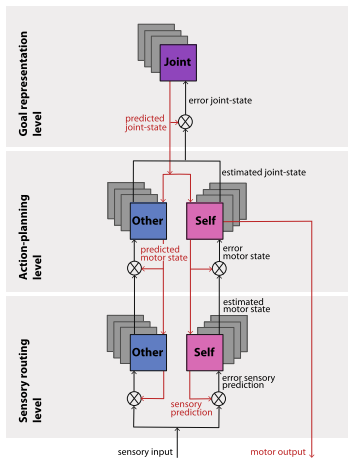
\includegraphics{images/PJAM.png}
      \caption{The Predictive Joint Action Model \citep{Pesquita2017}}
        \label{fig:PJAM}
   \end{center}
\end{figure}

PJAM assumes that each participant in a joint-action maintains internal models of themselves, their partners, and the joint task.  is composed of three hierarchical levels of inference: goal representation, action-planning, and sensory routing.

The goal-representation level of the model suggests that participants in joint action generate and monitor representations of the shared task. This proposal is formulated from evidence that musicians maintain shared representation of desired unified sound of an ensemble \citep{Keller2008}.  In one study using a neurophysiological measurement that codes unexpected events (ERP), Loehr and colleagues \textcite{Loehr2013} showed that musicians tracked deviations from a desired joint state;  in another study, Loehr and Vesper \textcite{Loehr2016} demonstrated that playing music together generates shared expectations regarding the desired state of joint action, and this process guides future action. Taken together, this evidence suggests that participants in joint action utilise prediction errors arising from lower levels to update representations of shared tasks.
%(Wolpert MOSAIC model doesn't account for updating rep. of shared task)

At the action-planning level, pairs of models represent the expected contributions to a joint-action of self and others. Action-planning entails, on the highest level, action roles (); on a mid-level, movement trajectories (); and on the lowest level, movement of muscle groups of self and others.  The action-planning level of PJAM is supported by evidence that participants in joint action generate internal models of self and other, known as co-representation  either spontaneously and involuntarily, as in the commonly used social simon task experimental paradigm \citep{Sebanz2003,Atmaca2008}, or more deliberately, as in the case of a coordinated dyadic horizontal jumping task \citep{Vesper2012}.  Studies show that co-representation is modulated by mood \citep[positive or negative affect, see][]{Kuhbandner2010}, self-concept and social orientation  \citep{Colzato2012,Colzato2012a}, and group membership \citep{deBruijn2008,Iani2013}.


As with goal representation, action-planning is a predictive process \citep{Flanagan2003}, in which individuals encode motor prediction errors concerning others' actions (in addition to their own) \citep{Vanschie2004,Radke2011}.  Predictive models of self and other action plans appear to be grounded in an individual's own motor simulation processes,  such that each participant maintains covert motor activations relating to expected contributions of their partners \citep{Hollander2012}.  Loehr and Vesper (2016) demonstrate that when learning a joint piano piece, musicians are able to better perform the piece together rather than solo, representations about each individual in a social interaction are encoded within the joint context of the interaction. In other words, when we learn a joint task we learn our own role and the impact of other's roles on our own role in the joint action.




The sensory routing level receives the inflow of sensory input and compares it to internal model predictions pertaining to each partner’s action outcomes within the inter-action. Each level generates predictions of the information that it expects to be found on the level below.  Continuous comparison between adjacent levels results in error signals that are sent up to optimise subsequent predictions in the level above.

humans rely heavily on assumptions about the internal processes of others (e.g., what they are feeling, thinking, and attending) to successfully align with others in space and time,

Individuals appear to draw heavily upon their own cognitive resources to build mental models of other people’s cognitive states

as well the perception of an implicit common ground and explicit shared goal to structure joint tasks.





Use the resources already proven effective for intra-personal coordination, and apply the same processes to joint action.

Series of hierarchically organised interoceptive predictive models, which are weighted by uncertainty (Bayesian inference)

In real world joint action scenarios such as sport, co-actors interact and rehearse their behaviours to produce a hierarchy of aligned representations, an implicit common ground on which joint action can unfold.

\subsubsection{Action-perception links}

            Action-perception links (MNN) etc




\subsubsection{Extra-neural direct coupling}

In interactive, cooperative tasks, individuals have been found to couple and reciprocally constrain their movements reducing the overall control needed to maintain effective cooperation \citep{Ramenzoni2011,Ramenzoni2012,Riley2011,Schmidt1990}.  Individuals’ behaviours become increasingly interdependent, so that a higher-level structure of the interaction emerges. This kind of emerging organisation has previously been referred to as soft-assembly \citep{Kello2009}: individuals preserve a degree of autonomy, but their behaviour is constrained by the interaction. They can flexibly engage and disengage from it, as well as become part of other soft-assemblies \citep{DeJaegher2010,DiPaolo2012}.




There is also evidence of extra-neural solutions to joint action problems, whereby agents achieve and sustain direct coupling with resources of the joint action environment, namely other actors and the physical resources of the task-specific environment.

      * CC motion:
      * Functional interpersonal synergies:
      * Schmidt and Richardson 2009
          * Can be measured by pink noise and multi-fractal analysis
      * (Bourbousson - Rowers and BBallers, go towards more efficient).

Direct coupling with the environment could set the foundation for more effective higher order processes of information transfer and communication.


\subsubsection{Individual differences}

Personality, social preferences (Keller & Novembre 2015),
Technical competence
Experience



\subsubsection{Culture}

FRAMING:
Joint actions that involve complex sequences and divisions of labour between participants appear to rely heavily on capacities to explicitly signal intention for the assigning of roles, forward planning, and repair of failed coordination \citep{Frith2010}. These ``coordination smoothers'' \citep{Vesper2017} often function to reduce spatial and temporal variation in action by providing a shared spatiotemporal referent for co-alignment of predictions.  Cultural conventions are examples of effective framing devices for joint action.  Depending on the context of the joint action, it could be subject to a pre-existing, mutually recognised power relation typical in the established culture (e.g., favouring hierarchical or egalitarian communication, \citep[see]{Cheon2011}) and the particular situational context (e.g., formal or informal).
Establishing roles, such as leader or follower, also has a similar smoothing effect, and often the affordances in the task environment shape the smoothing strategies available to co-actors \citep{Marsh2009}.


A key insight overlooked by the existing social high account of group exercise and social cohesion, but revealed by the paradigm shift surrounding the social cognition of joint action, is the sensitivity of joint action (or any cognitive process for that matter) to informational affordances provided by various layers of ecological and cultural context.  The cognitive inputs to joint action in real world settings are rarely limited to essentialise components administered in laboratory paradigms. It is known that cognitive processes relevant to joint action are distributed throughout brains, bodies, and the physical environment of the ecological niche in which it is situated.  There is evidence to suggest that joint action co-participants rely on a series ``frames of reference'' for joint action execution \citep{Ray2018}, and it appears that social interaction functions best in situations where there is a snug fit between individuals' implicit cultural expectations and explicit rules for engagement \citep{Vollan2017}.  Indeed, widespread attention to the ``reproducibility crisis'' in social science \citep{Earp2015,Rathmacher2017}, suggests that even the most controlled spaces and procedures of experimental studies involving human subjects are laden with unquantified and often culturally specific cognitive affordances that constrain and enable quantified outcomes.
%The experimental approach to science requires re-evaluation in light of an emerging paradigm emphasising distribution of cognitive processes throughout an array of coordinated informational affordances.

Discussed as part of the theoretical framework outlined in Chapter 2, shared cultural knowledge can act as a ``coordination smoother'' \citep{Vesper2017} for joint action, enhancing the effectiveness and efficiency of joint action between co-participants who share a similar informational framework.  In the predictive coding paradigm, cultural habits and frames of reference act as ``hyper-priors'' that set the macro-contextual coordinates for joint action\citep{Clark2013}.  Contextual affordances for joint action appear to be dictated by processes operating at multiple conceptual levels---from the micro-level predictive processes associated with movement action and perception, to the macro-level predictive frames offered by specific cultural and contextual niches---interact in complex processes of reciprocal causation to shape joint action (SOURCE).  Conceptualisation of the causal complexity of cognitive processes relevant to joint action in this way echoes a broader reconceptualisation of the causal complexity associated with change on an evolutionary timescale, which recognises that human behavioural phenomena is the result of a number of biological, cognitive, and ecological mechanisms that interact via reciprocal feedback loops spanning varying scales of time and space \citep{Fuentes2015}.




\subsection{Social connection through joint action?}


EMOTION:
cortical processes of prediction error management appear to be fundamentally mediated by the activity of the dopaminergic system \citep{Schultz2016}, while subcortical neuromodulatory systems, such as those responsible for producing norepinephrine, acetylcholine, and endogenous opioids, appear to be involved in attuning cortical processing to signals from the body and environment that are important for survival \citep{Lewis2005}.  There is now evidence to suggest that complex cognitive processes--- traditionally understood to be confined to cortical regions--- and subcortical neuromodulatory systems--- tradtionally understood to be responsible only for affective response and exogenous to the brain's inferential processes--- work in a loop of reciprocal interaction in order to enhance processes of error management \citep{Damasio1994,Lewis2005,Miller2017,Barrett2017}.
Emotions can in this sense be understood more as superordinate programs for regulating disparate subordinate cognitive modules for the purposes of global coordination with the environment \citep{Cosmides2000}.  By collapsing the common neurocognitive distinction between cortical and subcortical processes, PP, in addition to unifying perception, representation, and movement in a common theoretical framework, also helps integrate the role of affective processes into ``active inference.''

The distinction between cognition and emotion is supported by the idea that segregated brain areas implement cognitive and emotional functions and that there are two independent processing routes, one cognitive/controlled and one emotional/automatic, which usually compete (but also occasionally cooperate) to control behaviour \citep{Kahneman2003}.  However useful this ``dual-systems'' view has been thus far in cognitive science, prevailing evidence concerning the complexity of functional integration and segregation of brain processes challenges the cognitive-emotional distinction \citep{Pessoa2013}.  The emerging view is not only that cognition interacts with emotion at many levels, but that in many respects they are functionally integrated and continuously impact each other's processing.








\subsubsection{Prediction affect: positive violation of expectations}

A conscious sense of agency could be conceptualised within PJAM as a perceived match between higher level intentional action planning, and corresponding sensory effects at a lower level.

A hierarchical alignment of predictions and sensory input \citep{VanderWel2012}.

attributing sensory consequences to joint action partners is linked to cooperative success Chaminade2012, potentially via the parietal operculum (Goodbody and Wolpert 1998)





We have suggested that affect serves as feedback on our predictions, reflecting their accuracy and regulating them so that confirmed predictions are more likely to be used again (Chetverikov, 2014; Chetverikov & Kristjansson, 2015). Furthermore, if predictions are confirmed (lowprediction error), feed- back is weightedwith inverse prior probabilities of predictions, so that more probable predictions receive less positive feedback. In other words, confirmation of more probable predictions yields less positive feedback than confirmed less-probable predictions. Notably, within this framework there is no need to invoke additional concepts, such as values or rewards, to explain the relationship between affect and pre- dictions. Affect represents a distinct dimension in experience: in addi- tion to our “best hypothesis” about the world, people experience a feeling of howgood this hypothesis actually is. The literature describing affect fromthis perspective has largely been limited to the perception of art (Salimpoor, Zald, Zatorre,Dagher, &Mcintosh, 2014; van de Cruys & Wagemans, 2011).Wefill this gapbyproviding amore generalperspec- tivewithin a predictive coding framework.



Others form part of predictions and perceived outcomes

locus of control (locate agency in others/self)

















\subsubsection{Team Click}



Perception of direct








\subsection{A novel theory of social bonding through joint action}


\subsubsection{Predictions}

















































This approach to cognition offers the opportunity to re-examine of component mechanisms and system dynamics of interpersonal coordination.


Recent advances in neuroimaging technologies \citep{Frith2007}, emerging neurocomputational theories of brain function \citep{Friston2010,Frith2010,Clark2013}, and constructive attempts to extend the theoretical paradigm of human social cognition to account for inter-individual processes of interaction and coordination \citep{Sebanz2006,Dale2014},

 basal human capacities for physical movement regulation and coordination set the foundation for social cognitive systems whose resources are distributed between brains, bodies, and physical features of task-specific environments \citep{Hutchins2000,Kirsh2006,Semin2008,Semin2012,Coey2012}.



now provide an opportunity to address significant knowledge gaps within the cognitive and evolutionary anthropology of group exercise.   within this domain,


Furthermore, it has been shown that the quality of coordinated movement within these cognitive systems has implications for psychophysiological health and subjective well-being \citep{Wheatley2012}, and is relevant to the effective function of more complex goal oriented social activities, including the large-scale reproduction and transmission of shared cultural practices \citep{Dunbar2012,Roepstorff2010,Claidiere2014,Launay2016}. Thus, there is evidence to suggest that the ``visceral'' dimension of group exercise, traditionally occluded by theoretical convention and methodological challenges, can now be accessed by interrogating the ways in which cognitive mechanisms and system dynamics of joint action are responsible for processes of social cohesion.

A key facet of the paradigm shift in social cognition outlined above is the overhaul of traditional individual-centred computational models of information processing (originally inspired by the mechanics of the electronic computer), which tend to render movement as the final product of a linear sequence of sensory perception, amodal mental representation, and action selection \citep{Lewis2005}.  By contrast, the prevailing neurocomputational paradigm of ``predictive processing,'' also known as ``predictive coding,'' \citep[see][]{Frith2007,Kilner2009,Clark2013} offers a model of brain function in which perception, representation, emotion, and action are functionally and temporally integrated in the service of informational processes.  Perception, cognition, and action work closely together to minimise sensory prediction errors by selectively sampling, and actively sculpting, the stimulus array.







\myparagraph{Predictive Processing}
Predictive processing (PP) is an attempt to model the way that the brain processes information to produce perception and action. The PP hypothesis depicts a brain that is constantly in the business of predicting probable worldly sources of sensory signals, and adjusting action schemas in order to minimise the error of these predictions (or maximise the precision of these models). Predictive coding first emerged in cognitive science as an explanation for ``black box'' problem of perception, but has since been extended to account for the role of action in cognition \citep{Friston2010}.
The human brain confronts a black box problem when attempting to infer the causes in the external world with only partial and indirect access to that world via sensory input signals. This blindness to the precise nature of the world means that the most effective strategy available to the brain is to begin by generating an internal model of the world (no matter how rudimentary it may be initially) and then iteratively update that model in response to ``errors'' that arise from discrepancy between the model and the information from sensory inputs \citep{Frith2007}.

There is mounting neurocomputational evidence to suggest that this inferential strategy is supported in the brain by multilevel and hierarchical arrangement of cortical structures, which enable bi-directional cascades of information between levels.  Higher levels of the cortical hierarchy formulate models based on prior experience, which are employed to ``explain away'' sensory signals at lower levels. Lower level signals unaccounted for by higher level predictions are incorporated into higher level structures and strengthen the robustness of the model.  Predictive processing has been likened to a process of ``empirical Bayes,'' whereby prediction errors function to strengthen prior probability distributions of models for future inference \citep{Robbins1964}.  In a typically Bayesian manner, predictive processes appear capable of factoring representations of uncertainty around sensory signals into the predictive model itself \citep{Clark2013}.  The brain's capacity to quantify the uncertainty of any given sensory state facilitates optimal selection between competing predictions pertaining to the same bottom-up sensory signals, judged probabilistically.  At any one moment, an individual has access to multiple hypotheses derived from priors, which compete for the best fit of the sensation, until that process leads to fixation on the best hypothesis for the sensory state.
Binocular rivalry, (for example looking at a necker cube) is an instance in which there is insufficient sensory information available in order to reach fixation on one model over another (see Image ~\ref{fig:neckerCube} \citep{Frith2007}.

\begin{figure}[htbp]
  \begin{center}
    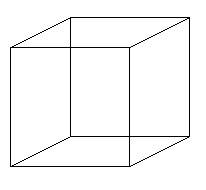
\includegraphics{images/Necker_cube.png}
      \caption{Necker Cube: The binocular rivalry is associated with insufficient sensory information}
        \label{fig:neckerCube}
   \end{center}
\end{figure}

\myparagraph{Active Inference}
Importantly, in the case of motor systems, the agents are able to move their sensors in ways that amount to actively seeking or generating the sensory consequences that they (or rather, their brains) expect.  In this way, ``error signals self-suppress, not through neuronally mediated effects, but by eliciting movements that change bottom-up proprioceptive and sensory input'' \citep[186]{Clark2013}. Perception, representation, and action functionally and temporally integrate to fulfil an ever evolving set of sub-personal expectations about the state of the world.  Perception, cognition, and action work closely together to minimise sensory prediction errors by selectively sampling, and actively sculpting, the stimulus array.

\myparagraph{Neurobiological underpinnings of PP and the role of emotion}
The PP hypothesis is also underwritten by a plausible neurobiological account. Specifically, the complex cortical processes of prediction error management appear to be fundamentally mediated by the activity of the dopaminergic system \citep{Schultz2016}, while subcortical neuromodulatory systems, such as those responsible for producing norepinephrine, acetylcholine, and endogenous opioids, appear to be involved in attuning cortical processing to signals from the body and environment that are important for survival \citep{Lewis2005}.  There is now evidence to suggest that complex cognitive processes--- traditionally understood to be confined to cortical regions--- and subcortical neuromodulatory systems--- tradtionally understood to be responsible only for affective response and exogenous to the brain's inferential processes--- work in a loop of reciprocal interaction in order to enhance processes of error management \citep{Damasio1994,Lewis2005,Miller2017,Barrett2017}.
Emotions can in this sense be understood more as superordinate programs for regulating disparate subordinate cognitive modules for the purposes of global coordination with the environment \citep{Cosmides2000}.  By collapsing the common neurocognitive distinction between cortical and subcortical processes, PP, in addition to unifying perception, representation, and movement in a common theoretical framework, also helps integrate the role of affective processes into ``active inference.''

The distinction between cognition and emotion is supported by the idea that segregated brain areas implement cognitive and emotional functions and that there are two independent processing routes, one cognitive/controlled and one emotional/automatic, which usually compete (but also occasionally cooperate) to control behaviour \citep{Kahneman2003}.  However useful this ``dual-systems'' view has been thus far in cognitive science, prevailing evidence concerning the complexity of functional integration and segregation of brain processes challenges the cognitive-emotional distinction \citep{Pessoa2013}.  The emerging view is not only that cognition interacts with emotion at many levels, but that in many respects they are functionally integrated and continuously impact each other's processing.

\myparagraph{The Free Energy Principle}
It has been suggested that the cognitive principle of error minimisation should be understood as a consequence of an overarching mandate of an organic system to minimise the informational degrees of freedom or ``free energy'' in that system's exchanges with the environment \citep{Friston2010}.  Thermodynamic free energy is a measure of the energy available to a system to do useful ``work'', i.e. work that contributes to the maintenance of system structure and organisation \citep{Stoner2000}.
Transposed to the cognitive domain, free energy emerges as the difference between the way the world is \textit{represented} as being, and the way it actually \textit{is}.
Thus, the better the model fit, the lower the information-theoretic free energy, or in other words, more of the system's resources are being put to effective work in representing the world.  In this formulation, ``surprisal'' (deliberately distinguished from surprise by Tribus \textcite{Tribus1961}) is a measure of sub-personally computed implausibility of some sensory state given a model of the world \citep{Clark2013}.  Entropy, in turn, can be understood as the long-term average of surprisal, or the informational cost for representing the sensory input by its internal model \citep{Little2013}.  Thus, good models of the world reduce surprisal and therefore achieve lower entropy.  The Free Energy principle draws attention to the fact that the brain's neurcomputational processes do not happen in isolation, but instead are embedded within larger biophysical and information-theoretical systems which constrain and direct their function.


Perception, cognition, and action work closely together to minimise sensory prediction errors by selectively sampling, and actively sculpting, the stimulus array.












\myparagraph{Functional interpersonal synergies}
For a brain in the business of prediction error minimisation, interpersonal interactions with other agents present a computational challenge due to the moving parts.  The large number of independently controllable movement system degrees of freedom of multiple agents places computational burden to the central nervous system, dubbed by Bernstein \textcite{Bernstein1967} as the ``degrees-of-freedom problem'' \citep[see also][]{Turvey1982,Turvey1990}.  From a system dynamics perspective, a solution to this problem is to work in such a way that the movement system degrees of freedom residing in different actors and environmental features are coupled to form low-dimensional, reciprocally compensating synergies, known as ``functional interpersonal synergies'' \citep{Riley2011}.

Much like intra-personal coordination, functional interpersonal synergies are temporarily assembled, task-specific, functional couplings between a system's componential degrees of freedom, such that one component of a synergy reacts to changes in the others \citep{Kelso2009}.  Once coordinated to behave as a functional unit, the individual degrees-of-freedom do not need to be controlled independently of one another, and perturbations applied to a component are automatically compensated by the coupled components \citep{Kelso1984,Latash2002,Riley2011}, making them adaptive responses to environments of high computational uncertainty.

Experimental evidence has shown that functional interpersonal synergies, for example in-phase or anti-phase coordination of hand movements, facilitates memory recall of incidental information concerning co-actors \citep{Miles2010}. It has also been shown that interpersonal synergies more generally facilitate performance of social cognitive or linguistic tasks, such as gaze coordination and turn taking in conversation \citep{Richardson2005,Shockley2009}.  Richardson and Dale (2005), for example, show that more tightly coupled gaze between conversing dyads leads to higher discourse comprehension.  Conversely, being psychologically distanced from another individual can inhibit the emergence of interpersonal synergies \citep{Miles2010}.  The ways in which functional interpersonal synergies facilitate adaptive information transfer between individuals and within groups suggests that psychological mechanisms and cultural practices responsible for generating these synergies could have been subject to cultural evolutionary forces of selection and attraction \citep{Claidiere2014,Mesoudi2016a}.

Considered form within the PP and Free Energy principle paradigms, interpersonal synergies represent one way in which error minimisation can be achieved via extra-neural mechanisms.  In addition to the behavioural mimicry and synchrony literatures mentioned above, research into the coordination dynamics of natural joint actions has shown evidence of dynamic coupling (functional synergy) in joint action tasks, such as dancing, martial arts, moving objects like furniture.  In studies involving skilled versus non-skilled practitioners in dyadic interactions, it has been shown that more skilled practitioners create stronger dynamical coupling through flexibly modulating their actions with others \citep{Schmidt2011, Caron2017}. These findings are corroborated by other studies that find that professional footballers (versus novice controls) are able to more accurately predict the direction of a kick from another player's body kinematics (\cite{Tomeo2012}, see also \cite{Aglioti2008,Mulligan2016} for similar results with basketball and dart players). Interestingly, when analysing co-regulation between members of basketball teams, it was shown by Bourbousson \textcite{Bourbousson2015} that more expert teams made fewer mutual adjustments (at the level of the activity that was meaningful for co-actors), suggesting an enhanced capability of expert social systems to achieve and maintain an optimal level of awareness during the unfolding activity, potentially implicating down-regulation of prediction error management processes.










Literature suggests that successful joint action in humans is contingent on the ability to share functionally equivalent task representations. Considering the cognitive principles of ``active inference'' referenced above, shared task representation amounts to minimising prediction error in social cognitive systems involving two or more co-actors \citep{Semin2008,Frith2010}.  Humans appear to employ an array of explicit and implicit behavioural strategies in order to achieve this.  The ways in which co-actors ``close the loop'' \citep{Frith2007} on joint action through deliberate ostensive communication has been the traditional focus of developmental, comparative \cite{Tomasello2005a}, and social psychologists \citep{Sebanz2006}.

More recently, however, analysis of dynamic coupling of co-actors in joint action scenarios reveals that synchronised movement implicates an array of implicit and pre-perceptual cognitive processes of alignment and prediction error minimisation \citep{Schmidt2011}, which, in addition to more explicit forms of communication, could be central to the generation of feelings of self-other merging, self-other distinction, and perceived reliability and trust associated with social bonding \citep{Marsh2009}.


\myparagraph{Specialised Mechanisms of Joint Action}
\myparagraph{Predictive Coding & Thermodynamics of cognition}
\myparagraph{Functional Interpersonal Synergies}
\myparagraph{Affect and prediction: expectation violation as mechanism}
\myparagraph{Moderators}






\clearpage
\section{Existing evidence for a relationship between joint action and social bonding} %1361


Considering this dissertation's specific theoretical focus on the relationship between proximate mechanisms of group exercise and their effects of team click and social bonding, the social cognition of joint action provides the most appropriate entry point for analysis.  Joint action, broadly construed according to the definition above, encompasses various areas of empirical research, including behavioural synchrony \citep{Reddish2013,Launay2016,Mogan2017} and nonconscious mimicry \citep{Bargh2012}---the bonding effects of which have been clearly demonstrated.  Real world instances of joint action also encompass less tightly coupled forms of interpersonal coordination, such as those found in interactive team sports, music-making, and in dance.  The social dynamics of these joint action scenarios are only just beginning to be analysed theoretically, experimentally, and observationally \citep{Marsh2009}.

Extensive research within developmental, comparative, and social psychology demonstrates that various cognitive, sensorimotor, affective, and cultural processes underpin the ability and desire to establish and maintain joint action.  As such, the mechanisms responsible for feelings of team click and social bonding through joint action may also be various and diverse.

On a fundamental level, joint action depends on the abilities to 1) develop functionally similar representations of a shared task between two or more individuals, and 2) anticipate and integrate the effects of own and others' actions in the representation of a joint action\citep{Sebanz2006a}.

The cognitive mechanisms that underpin these abilities can be organised into three main categories: 1) mechanisms that enable shared task representations, 2) mechanisms that facilitate the formation and maintenance of functional interpersonal synergies between co-actors, and 3) mechanisms that serve to contextually frame joint action, such as internalisation of explicit cultural conventions\citep{Sebanz2006,Vesper2017}.  Ethnographic and experimental evidence suggests that positive psychological and social effects of joint action are most pronounced when these specific component mechanisms are maximally activated \citep{Durkheim1965,McNeill1995,Mogan2017}.  Tightly coupled (i.e., time- and phase-locked) coordination of movement known in the literature as behavioural synchrony (hereafter synchrony), is recurrent in many cultural practices including music making, dance, sport, and military drills, and its behavioural effects include prosociality, perceptions of social bonding, and positive affect \citep{Mogan2017}.  The fact that the link between synchrony and social bonding is most closely analysed may indeed be associated with the fact that joint action in these scenarios is hightly accentuated and idealised to facilitate successful coordination.  Synchrony is a predictable and cheap coordinator of behaviour, and is easily scalable to the coordination of behaviour in large groups, which may explain its cross-cultural ubiquity in cultural practices \citep{Dunbar2010,Tarr2016}.

However, similar social effects and process mechanisms appear to take place in other joint action scenarios in which movement is not as tightly, predictably, or deliberately coupled.  Experimental research on non-conscious mimicry indicates that positive social effects such as liking, rapport, and cooperation are observable when participants ether mimic others or unwittingly are mimicked by a confederate, but not when participants are made consciously aware that the mimicry was taking place \citep{Bos2008,Lakin2008}.  In addition, dynamic coupling has been shown to exist in more complex dyadic and group joint action scenarios, such as those found in martial arts \citep{Schmidt2011}, music performance ensembles \citep{Demos2014}, sub-phases of interactive team sports \citep{Duarte2013}, and group dancing \citep{Chauvigne2017}. These studies find evidence of complex multi-scale ``fractal-like'' coordination of action between co-participants, often existing at the pre-perceptual level of awareness \citep{Schmidt2011,Riley2011,Fusaroli2013}. While behavioural synchrony has understandably received the most attention from experimental social psychology (presumably due to the ease in which it can be experimentally manipulated), less tightly controlled forms of joint action have been much less closely scrutinised for evidence of their social and affective dimensions\citep[but see]{Marsh2009,Miles2009}.  This is a clear theoretical and empirical gap in the social cognition of joint action; one which I seek to address in this dissertation.

\subsubsection{Neurocognitive and physiological mechanisms linking synchrony and social bonding}
In order to address this gap in the literature concerning the social dimensions of real-world joint action, it is necessary to begin by assessing the existing literature, which predominantly focusses on the social effects of tightly coupled behavioural synchrony. Three mechanisms have been identified as underpinning the various social effects of synchrony \citep{Lang2017,Mogan2017}.  First, synchrony has been associated with the phenomenon of ``self-other merging,'' whereby synchronous activity blurs the perceptual or phenomenological boundaries between self and other/group agency, possibly due partly to exact action-perception matching of synchronised activity \citep{Hove2008}.  Second, it has been proposed that synchrony enhances group-centred cognition, whereby attention to the actions of others enables the calibration of behaviours and enables the rehearsal of cooperation. Group centred cognition is thus often operationalised as perceived cooperation between co-participants \citep{Reddish2013}.

Third, synchrony appears to be responsible for activating an affective physiological mechanism, which has been associated on the one hand with feelings of calm, euphoria, and positive affect, and on the other hand with prosocial behaviours such as decision making in economic games and spontaneous helping \citep{Wiltermuth2009,Reddish2013a,Mogan2017}.
It has been proposed that this synchrony-activated affective mechanism is neuropharmacologically mediated, the primary candidate being the endogenous opioid system.  Unfortunately, due to the blood-brain barrier in humans, direct measurement of endorphins is difficult, requiring invasive and expensive methods.  As such, the ``endorphin hypothesis'' in coordinated and exertive human group activity is operationalised in experimental settings by measuring pain threshold, an indirect, proxy method. \citep{Dunbar2008,Sullivan2013,Sullivan2014,Tarr2015}.

Importantly, it also appears that for these three mediating mechanisms of synchrony, ``group-size matters.'' In the case of self-other merging and group-centred cognition mechanisms---which are both predominantly neurocognitive accounts---results appear to be strongest in synchrony experiments involving dyads and small groups, for which the attentional requirements for tracking co-participants is within healthy adult human capacity \citep{Mogan2017}.The affective (endorphin-mediated) pathway between synchrony and social bonding, by contrast, appears to function effectively in larger group settings, in which the cognitive load associated with tracking and attending to specific co-actors in joint action is more burdensome.  In these settings, prosocial behaviour and social bonding is generalised beyond specific individuals and often attributed to the group as a whole, or to other targets such as the environment (biophillia) \citep{Reddish2013b, Reddish2016}.

A recently published experiment designed to systematically assess the relationship between these three hypothesised mediators and the social effects of synchrony found that synchronisation between individuals (a series of waving arm movements) positively activated all three mediating mechanisms (self-other merging, group-centred cognition, and higher pain threshold), and led to higher levels of liking and prosocial behaviour (measured by contributions to the confederate in a ``trust'' economic game) \citep{Lang2017}.  Interestingly, the likeability and economic game measurements were uncorrelated, and path analysis revealed that self-other merging and group-centred cognition displayed high predictive power
in mediating the effects of synchrony on likeability but not on behaviour in the economic game.  The affective mechanism (measured by pain threshold), by contrast, exhibited a significant positive relationship between pain threshold increase and both likeability and economic game investment.  Combining all three pathways in one model resulted in two statistically significant paths: one involving pain-threshold increase to higher investments; and another through group-centred cognition to likeability of the interaction partner.  These results thus support a distinction between the neurocognitive and physiological aspects of synchrony, and suggest that neurocognitive mechanisms of synchrony enable ``cognising in the we mode'' \citep{Gallotti2013,Hasson2016,Kirschner2010}, whereas physiological processes might play a crucial role in economic decision-making, perhaps by helping reduce the inherent stress involved in social interaction \citep{Mogan2017,Kret2015,Stanley2011}. This research indicates that various distinct but complementary mechanisms may work in concert to generate the social effects of synchrony.  Indeed, it should also be expected in the case of less tightly coupled instances of joint action, such as those found in competitive interactive team sports, that various distinct but complementary mechanisms may work in concert to generate the social bonding effects.



\subsubsection{Applicability of synchrony-induced mechanisms of social bonding to joint-action, and their relevance to team click}
For the purposes of this dissertation it is important to consider to what extent these mechanisms are applicable to the study of joint action beyond the tightly matched behaviour of synchrony.  In particular, I will pay attention to mechanisms that appear most relevant to the observable phenomenon of team click. While neuropharmacologically-mediated affective mechanisms of synchrony are very relevant to joint action and social bonding in group exercise contexts \citep[see]{Cohen2009,Sullivan2013,Tarr2015}, the phenomenology of ``team click'' suggests that the perceived \textit{quality} of joint action with co-actors is also relevant.  Thus, in dynamic joint-action scenarios, (neuro)cognitive mechanisms of perception and action may facilitate psychological affiliation and social bonding.  Furthermore, there is evidence to suggest that traditional distinction between physiological (affective) mechanisms and neurcognitive mechanisms of joint action should be re-evaluated based on emerging neurocomputational theories of brain function and theories of distributed social cognition \citep{Pessoa2013,Pessoa2014,Miller2017}.


\myparagraph{Mechanisms of joint action}
It is generally understood that establishing and maintaining commitment to joint action, depends on an ability to somehow share a functionally equivalent representation of the joint task\citep{Vesper2010,Michael2016}.  BT: clarify how mimicry fits in with shared representation of joint actions before exploring the developmental evidence below.

Evidence for the ability to form and commit to shared tasks can be identified in infant development.  New-borns and infants engage in dyadic relationships in which imitation and other proto-conversational communicative behaviours emerge in a symmetrical and contingent fashion with carers (also known as ``motherese,'' see \cite{Braten2007}). At the age of approximately 9 months, more complex multi-agent ``triadic'' interactions can be sustained \citep{Colle2008}, seemingly underpinned by an enhanced capacity to maintain joint attention.
In experimental settings, infants demonstrate a precocious tendency (compared to captive non-human primate adults) to imitate the actions of authoritative others \citep{Tomasello2014}, and are known to be highly susceptible to automatic processes of motor and emotional contagion and entrainment \citep{Bargh2012}. The mechanisms that underpin these examples of early life joint action confer obvious adaptive benefits, and, as demonstrated in the nonconscious mimicry and behavioural synchrony literatures, appear to be directly tied to neurobiological reward mechanisms and prosocial behaviours \citep{Hurley2008,Launay2016}.

Joint action requires mechanisms that not only generate shared task representations, but also those that facilitate the on-line monitoring and updating of representations such that they are adaptively calibrated to the representations of co-actors, and to the task-specific environment.  Whether it is a physical piece of furniture that is being moved, or an abstract mental concept that is the object of discursive ``movement'' in a spoken conversation or written exchange, joint action demands the ability to coordinate attention and communicate sensorimotor information relevant to a common focal point.  The basal human capacity to maintain joint attention to a common object (which starts to emerge by 9-12 months in infants, \cite[see]{Carpenter2013}) underwrites higher order and the elaborate process of sharing attention around mental representations and articulating explicit common goals \citep{Tomasello2014}.
Humans are particularly adept, even from a very young age, at attending to biological motion \citep{Scholl2000}, especially when it carries socially-relevant information \citep{Kozlowski1977,Cutting1977,Dittrich1996}.
We are capable of reading others' affective states from body movements, body posture, gestures, facial expressions, and action performance, possibly via activation of the observer's corresponding states \citep{Bastiaansen2009,Borgomaneri2012}. Sharing emotions with others provides motivational cues helpful to initiate and continue joint tasks and to facilitate coordination \citep{Michael2016}. Existing evidence suggests that the communicative function of emotions may operate via a two system model which distinguishes between automatic reflexes-based manifestations of an emotional message and more deliberate emotional expression based on reflection and decision-making\citep{DeGelder2006}.

\myparagraph{Self-other merging}
The well-documented experience of synchrony-induced self-other overlap, associated with a distribution of agency to co-participants and a ``sense of oneness with the group'' \citep{Swann2012} does appear to be relevant to the experience of ``team click'' and joint action more broadly.  The flow literature consistently documents reports from athletes, musical performers, and other expert practitioners that involve a ``loss of self'' and an extension of agency to joint-action co-participants \citep{Jackson1995,Jackson1999}.  However, it is not yet clear via what mechanisms self-other merging is generated in these activities, and which of these mechanisms in particular is most applicable to the phenomenon of ``team click.''

Controlled experiments have demonstrated that simultaneous activation of one's own muscles and the observation of others behaving in an identical way leads to a blurring of the self and other in the mind of the individual \citep{Hurley2008,Rizzolatti2004}. These findings are consistent with the suggestion that coordination observed between agents in joint action relies on the  mirror neuron system, which enables the execution of similar but independent motor programs co-activated by a direct link between action and perception \citep{Rizzolatti2004}.  While this interpretation of self-other merging is parsimonious with exact matching of action and perception common in behavioural synchrony, it is less applicable to an explanation of the extension and blurring of agency that occurs in joint action that does not involve direct action-perception matching. Indeed, results of self-other overlap-mediated bonding effects of synchrony are in fact mixed, with some studies failing to find a direct relationship \citep{Cohen2013a,Reddish2013a}, and replications of seminal studies have failed to reproduce effects of cooperation or perceived social bonding \citep{Dam2012,Schachner2010}.\footnote{Schachner and Garvin (2010), for example, conducted a direct replication of Wiltermuth and Heath's (2009) third study and found that synchrony did not increase cooperation, nor perceived social bonding (i.e., trust, similarity and feelings of being in the same team.} It is plausible that other cognitive mechanisms may be at play in both exact synchrony and joint action more broadly.

%(BT: When I was writing up I was cautioned against using the term Mirror Neurons, and to rather stick with phrases like ‘co-activation of perception and action networks’, merely because there is a lot of literature that uses the term ‘mirror neurons’ with regard to other more higher order effects, around which I believe there is still a lot of debate about the robustness/interpretability of these results. This can just derail the conversation/distract from what you are trying to communicate. That said, I think it would be fine (and not necessarily incorrect) to refer to the mirror neuron system here, but you may need to clarify exactly what it is a bit better than you have done in this sentence. E.g. look for some more recent references to ensure you have a solid up-to-date description of what you are describing. (maybe see Kilner & Lemon 2013, who say “ Mirror neurons were originally defined as neurons which “discharged both during monkey’s active movements and when the monkey observed meaningful hand movements made by the experimenter” [2]. Thus, the key characteristics of mirror neurons are that their activity is modulated both by action execution and action observation, and that this activity shows a degree of action specificity. This distinguishes mirror neurons from other ‘motor’ or ‘sensory’ neurons whose discharge is associated with either execution or observation, but not both. It also distinguishes mirror neuron responses from other types of response to vision of objects or other non-action stimuli.” , but I note that they do not focus on human studies in this review).

%Perhaps see Caramazza et al. 2014.
%I flag this more for potential reviewers of papers, but also possibly Natalie will dig into this a little deeper. (see how she refers to the action perception network description in her papers as a hint of her standing? You could get away with just saying what you have said here, but it can be a polarising topic/term.)

Accumulating experimental evidence suggests that, in addition to direct action perception (BT: Be aware of action perception vs. action-perception) mechanisms, interoceptive (internal) representations of action-oriented motor programs also play a mediating role in successful coordination in joint action \citep{Moreau2016}.  Interoceptive representation of joint action has been shown to occur when a partner is absent but believed to be acting in another room \citep{Milward2014}, or when a partner is present but their actions are occluded \citep{Atmaca2011}, suggesting that individuals do not simply rely on a direct action-perception coupling, but also internally generate motor programs including the roles of co-actors in these shared motor tasks.
Evidence suggests that the neural signature of action planning is modulated when one's own action is part of a joint plan, compared to performing a corresponding solo or bimanual action, which indicates that neural representation of joint action is distinct from that of individual action, and may be indicative of a broader (extra-neural) cognitive system with dimensions and resources that are unique to joint action \citep{Kourtis2014}.

%Interestingly, evidence that joint activities involving joint attention (but not an explicit joint goal) produce higher levels of liking and social bonding than the same activity with an explicit joint goal (but no shared attention) (Wolf et al. 2016), suggests that basal capacities for behavioural synchronisation and alignment could be more closely related to the affective dimensions of collective movement than higher-order explicit processes of coordination\citep{Dunbar2008,Marsh2009}}.

\myparagraph{Grounded representations}
BT: more E and SIGNPOSTING HERE

1. MOTOR SIMULATION
It is thought that representations of cognitive systems generated in joint action scenarios are grounded in and constrained by 1) actors' intra-individual sensorimotor representations and 2) the specific extra-personal context of the joint action \citep{Sebanz2006}.  This has been demonstrated experimentally by contriving joint action situations involving little or no online perceptual information about the co-actor, for example coordinating the landing of a horizontal jump with an occluded co-actor \citep{Vesper2012}. When compared to an equivalent intra-individual coordination task (a bi-pedal coordination of a horizontal jump), similarities between intra- and inter-individual coordination dynamics suggest common mechanisms underlying both \citep{Schmidt2008}.  Thus, it follows that shared task representations in joint action also rely on scaffolds sourced locally, from an individual's own sensorimotor processes and immediate environmental affordances\citep{Williams2009}.


Frith and Frith \textcite{Frith2010} suggest that humans have evolved a particularly strong propensity to assign agency from perception of biological motion (known in evolutionary psychology as the Hyperactive Agency Detection Device or HADD, see \cite{Barrett2000,Barrett2007}), which could explain a tendency seen in religious practices to misattribute agency to supernatural agents \citep{Atran2010}.  Likewise, the misattribution of agency to teammates due to their contribution to shared task representations could also be a plausible explanation for ``feelings of oneness with the group'' experienced by athletes when they ``feel the click'' of joint action \citep{Swann2009}. The equivalence between feelings of self and distributed agency owing to common neurophysiological architecture underpinning both representations, may provide the psychological basis for social bonding in joint action.  Considering this evidence, it appears that self-other merging, common to the experience of behavioural synchrony and coordinated joint action more generally, relies on a range of cognitive mechanisms beyond exact behavioural matching.

\myparagraph{Self-other distinction}
Exact imitation of the actions of others is, of course, not always an adaptive approach to joint action.  The successful execution of complex joint actions also relies on a higher order ability to \textit{differentiate} between the actions of self and other and the translation of co-actors' roles in joint action into self- and task-relevant information \citep{Novembre2012,Sowden2014,Milward2016}.
The ability to cognitively process the fact that another actor may hold an attitude or intention that is contradictory to one's own emerges as an implicit (pre-declarative) capacity in infants from as early as 7 to 9 months \citep{Baron-Cohen1991}, before an explicit (declarative) capacity (known as ``formal ToM'') emerges between the age of 3-5 years. Concomitant with acquisition of more complex grammatical structures of spoken language, formal ToM allows humans to dynamically execute role-reversible and goal-directed action plans \citep{Tomasello2005a,Tomasello2008,Tomasello2014}.  Self-other differentiation in joint action appears to generate positive psycho-social effects.  de Guzman and colleagues \textcite{DeGuzman2015}, for example, showed that participants trained to increase self–other control in the motor domain demonstrate increased empathic corticospinal responses and self-reported empathy, as well as an increased ability to control imitation of others.
BT: I wonder whether this section shouldn’t come earlier? I.e. first explore the ability to distinguish self from other, then give some air-time to the descriptions of how merging of this representation etc arise and function.

\myparagraph{Contextual framings for joint action}
Joint actions that involve complex sequences and divisions of labour between participants appear to rely heavily on capacities to explicitly signal intention for the assigning of roles, forward planning, and repair of failed coordination \citep{Frith2010}. These ``coordination smoothers'' \citep{Vesper2017} often function to reduce spatial and temporal variation in action by providing a shared spatiotemporal referent for co-alignment of predictions.  Cultural conventions are examples of effective framing devices for joint action.  Depending on the context of the joint action, it could be subject to a pre-existing, mutually recognised power relation typical in the established culture (e.g., favouring hierarchical or egalitarian communication, \citep[see]{Cheon2011}) and the particular situational context (e.g., formal or informal).
Establishing roles, such as leader or follower, also has a similar smoothing effect, and often the affordances in the task environment shape the smoothing strategies available to co-actors \citep{Marsh2009}.

\subsubsection{Group-centred cooperation}
The evidence outlined above suggests that humans have evolved a suite of cognitive mechanisms that facilitate robust variation in strategies of merging with, and differentiation from, others for the purposes of adaptive joint action. In what ways do these mechanisms reward successful joint action, and how do these processes vary by activity and culture?

Given the diversity of mechanisms that appear to contribute to the social effects of joint action, the neurocognitive mechanism of group centred cognition---identified in the synchrony literature---could provide a useful framework for understanding the processes through which joint action generates social bonding.  Recent evidence suggests that the most powerful social effects of joint action are achieved when an explicitly shared goal is complemented and enhanced by perceptions of synchrony between co-actors \citep{Frith2010,Reddish2013}.
In this sense, synchrony is not simply the matching of behaviours but an outcome of, and an input to, joint action with consequences for cooperation and social bonding \citep{Keller2014,Lumsden2012,Obhi2011}.
Reddish and colleagues \textcite{Reddish2013} utilise path analysis to empirically substantiate the role of explicit and implicit cognitive processes in joint action.

The ``reinforcement of cooperation model,'' proposes that the social bonding effects of synchrony can be explained by the way in which synchronised behaviour implicitly enhances perceptions of successful cooperation, which in turn improves confidence and trust between co-actors, and then transfers to future cooperative tasks.  Further evidence suggests that the \textit{perceived} success of a synchrony task is a critical predictor of cooperative behaviour in economic games, more so than the precise matching of movements\citep{Kurzban2001,Launay2013}.  In other words, more important than the actual quality of coordination in joint action might be the extent to which synchronisation in a specific joint action task aligns with co-actors' \textit{expectations} for that task.  The reinforcement of cooperation model accords well with the dimension of team click, described above, pertaining to forging trust and perceptions of reliability between co-actors in joint action.
The highly visceral experience of movement coordination in joint action could function as a powerful signal of commitment and cooperation---a communication that one is trustworthy and competent enough to join another and fight ``in the trenches,'' for example.



\myparagraph{Prediction and expectation in joint action}
The alignment of co-actors' representations of joint action, via direct action-perception matching, or through the generation of functionally equivalent interoceptive shared-task representations, requires as a foundation the ability to anticipate or predict the actions of others.  In addition to prediction, sensitivity and attention to sensorimotor information available online in the task environment is crucial for the process of monitoring and updating shared task representations. Shared task representations appear to undergo a process of refinement, through an iterative process in which predictions about the consequences of partner-generated actions are tested against actual sensory inputs, with residual prediction errors in this fitting process being integrated into an updated shared task representation \citep{Vesper2016}. While joint action and synchrony literatures occasionally allude to the role of prediction in coordinating joint action on this level of technicality \citep[see for example][]{Sebanz2009,Glover2017}, prevailing theories of brain function and social cognition are yet to be fully incorporated into an account of joint action.  In particular, the neurocognitive processes and system dynamics of information transfer in social interaction suggests a model of joint-action in which predictive interoceptive models of joint action interact and synergise depending on their functional equivalence in cognitively distributed task-specific environments. In this sense, the ``click'' of joint action could be associated with the extent to which prediction is optimised in a cognitive system involving joint action coordination.  In the following section I suggest that a theory of social bonding through joint action in group exercise contexts such as rugby union must incorporate these prevailing theories in order to fully account for the phenomenon of team click.

%In the same way that sub-personal action prediction can structure the perception (e.g., Springer et al., 2011), studies have shown that top-down expectations about a co-actor's intentions affect perception in joint-action (Hudson et al., 2016a,b).
\clearpage



%~\ref{introduction}
\section{Grounding joint action and social bonding in the social cognition of physical movement}
In this section, I suggest that in order to account for the relationships between joint action, team click, and social bonding, a theory of social cognition grounded in the system dynamics of basal human capacities for physical movement is required. Biological and cultural evolutionary processes have facilitated remarkable transformations in human brain function from its humble mammalian beginnings. But, it is also important to keep in mind that the first ever problem solved by the mammalian brain was regulating physical movement, because physical movement remains its basal logic, even in humans who now at least \textit{appear} to be more preoccupied in day-to-day life with higher-order cognitive abstractions.  The basic design of the human brain was largely evident in simpler animals that had to solve the basic problems of survival in situated environments \citep{Pezzulo2014}.
\end{mccorrection}

As outlined above, steady improvements in neuroimaging technologies \citep{Frith2007} and neurocomputational theories of brain function \citep{Friston2010,Frith2010}, and attempts to extend the theoretical paradigm of cognition to encompass and satisfactorily account for inter-individual processes of interaction and coordination \citep{Sebanz2006,Marsh2009,Dale2014}, has directed attention to the ways in which automatic movement strategies anchor information transfer within and between individuals, groups, and throughout populations across space and time.  This amounts to a paradigm shift for cognitive science, and helps re-conceptualise cognition as a system situated in and distributed throughout human brains, conscious minds, active bodies, and feature-rich physical environments \citep{Wilson2013}.

Traditional individual-centric computational models of cognition, which tend to render movement as the product of a linear sequence of sensory perception, internal mental representation, and action selection, have been superseded by newer theories in which perception, representation, emotion, and action are functionally and temporally integrated in service of highly distributed processes of information regulation and transfer \citep{Clark2013}.  Conceiving of social cognition in this way, as an embodied, embedded, and immediate process of inference, centralises the role of automatic movement regulation strategies---traditionally classed as ``lower-cognitive'' processes---in establishing and maintaining the transfer of information between individuals, within groups, and throughout populations---traditionally thought to be executed by  ``higher-cognitive'' processes \citep{Claidiere2014}.

%In addition, traditional individual-centric computational models of cognition have been superseded by newer theories. Individual-centric models tend to render movement as the product of a linear sequence of sensory perception, internal mental representation, and action selection (see for example, SOURCE). On the contrary, newer models of cognition conceptualise perception, representation, emotion, and action as functionally and temporally integrated, all in the service of informational processes situated in—but also distributed throughout—human brains, conscious minds, active bodies, and feature-rich physical environments.

%Conceiving of social cognition as embodied and embedded centralises the role of automatic movement regulation strategies---traditionally classed as ``lower-cognitive'' processes---in establishing and maintaining the transfer of information between individuals, within groups, and throughout populations---traditionally thought to be the primary domain of ``higher-cognitive'' capacities \citep{Claidiere2014}.

From this emerging area of research, 5 core principles are relevant to the social cognition of joint action and social bonding, and as such serve as a theoretical foundation for the present study:

1. Human cognition is generated by a multitude of cognitive mechanisms responsible for regulating movement, evidence for which can be identified in a spectrum of social behaviours ranging from more explicit and deliberate communicative signals, through to more implicit (often pre-perceptual) processes of synchronisation and alignment of the organism with the environment \citep{Frith2010,Semin2008}. Prevailing models of social cognition reveal that higher order explicit communication strategies traditionally privileged in computational accounts of cognition (e.g. consciousness, symbolic language, rational thinking), draw on only a small fraction of the total amount of information processed by the nervous system at any one moment \citep{Semin2012}.

2. Human cognition entails ``active inference'' \citep{Friston2010} about the world. Agents generate interoceptive predictions about the state of the world and test these representations against actual bottom-up sensory evidence \citep{Clark2013}.  In this conception, known as the predictive processing (PP) hypothesis, the fundamental drive of human cognition is to minimise ``prediction error,'' or the discrepancy between predictions of the world and the bottom-up sensorial experience of the world. In PP, perception, representation, emotion, and action are unified by the logic of prediction-error management, where neurocognitive components work together to align the organism with its expectations and in so doing produce adaptive behaviours \citep{Pezzulo2014}. Related to principle 1, much of the work of predictive processing occurs beneath the level of conscious awareness \citep{Frith2007,Clark2013}.
PP appears to be driven by reward mechanisms of neuromodulatory systems, namely the dopaminergic \citep{Schultz2016} and opioidergic \citep{Laurent2014} systems.  In addition, however, the embeddedness of neurocognitive processes in broader information-theoretic systems (discussed in principle 3 below) suggests that PP is also determined by a overarching mandate to reduce ``free energy'' (or entropy) in the nervous system's interaction with the environment \citep{Friston2010}.

3. Human cognition relies on resources that are distributed across neural, bodily, and environmental features of the social and physical environment, supporting action and interaction \citep{Hutchins1995,Kirsh1995,Smith2004}.  The embedded and distributed nature of cognition is observable in instances of joint-action, where the time-locked coordination of behaviour with two or more individuals in a physical environment gives rise to functional interpersonal synergies \citep{Riley2011,Coey2012}.  These coordinative structures reduce the degrees of freedom of the system components and allow for cognitive resources to be efficiently distributed across all nodes of the emergent dynamical system. The self-organising properties of dynamic coupling in joint-action have been modelled, revealing evidence of multi-scale fractal synchronisation and complexity matching \citep{Schmidt2011,Richardson2012}.

4. Higher quality synchronisation of behaviours in joint-action scenarios has positive implications for individual psychophysiological function, health, and subjective well-being \citep{Wheatley2012}.  In particular, successful coordination in joint-action has implications for psychological processes relating to social bonding \citep{Marsh2009,Launay2016}.  Evidence from the self-report of highly skilled joint-action practitioners (musicians, performers, athletes) suggests a strong link between the perception of high-quality joint-action and psychological well-being \citep{Jackson1995,Jackson1992}.  Conversely, the psycho-social isolation and ill-health experienced by individuals who suffer from developmental and neurocognitive deficits in behaviours key to dynamic interpersonal interaction is also well-documented \citep[e.g.][]{Blakemore2005,Baron-Cohen1991}.

5. The coupling dynamics of co-present joint action have implications for higher order and more complex goal oriented settings, including the re-production and transmission of shared cultural practices \citep{Dunbar2012,Roepstorff2010,Claidiere2014}.
%expand here...Dunbar's work on group network size online etc?



\subsection{Predictive Processing, Active Inference, and the Free Energy Principle}
A key facet of the paradigm shift in social cognition outlined above is the overhaul of traditional individual-centred computational models of information processing (originally inspired by the mechanics of the electronic computer), which tend to render movement as the final product of a linear sequence of sensory perception, amodal mental representation, and action selection \citep{Lewis2005}.  By contrast, the prevailing neurocomputational paradigm of ``predictive processing,'' also known as ``predictive coding,'' \citep[see][]{Frith2007,Kilner2009,Clark2013} offers a model of brain function in which perception, representation, emotion, and action are functionally and temporally integrated in the service of informational processes.



\subsection{Functional Interpersonal Synergies}
Explaining active inference within a larger framework of free-energy minimisation in a system's exchanges with the environment is in line with a broader recognition of the ways in which complex biological and information-theoretic systems both support and constrain processes of human social cognition \citep{Dale2014}.  The human brain, body, and the various functional behavioural synergies that humans form in social interaction, are all examples of dynamical systems of varying scales, whose physiological and cognitive parameters enforce constraints on the expression of their componential mechanisms.  Situating the activity of the brain in the constraints inherent in real-time and online social interactions is necessary for a full appreciation of the nervous system's role in the organisation of social behaviour and cognition \citep{Coey2012}.

For a brain in the business of prediction error minimisation, interpersonal interactions with other agents present a computational challenge due to the moving parts.  The large number of independently controllable movement system degrees of freedom of multiple agents places computational burden to the central nervous system, dubbed by Bernstein \textcite{Bernstein1967} as the ``degrees-of-freedom problem'' \citep[see also][]{Turvey1982,Turvey1990}.  From a system dynamics perspective, a solution to this problem is to work in such a way that the movement system degrees of freedom residing in different actors and environmental features are coupled to form low-dimensional, reciprocally compensating synergies, known as ``functional interpersonal synergies'' \citep{Riley2011}.
Much like intrapersonal coordination, functional interpersonal synergies are temporarily assembled, task-specific, functional couplings between a system's componential degrees of freedom, such that one component of a synergy reacts to changes in the others \citep{Kelso2009}.  Once coordinated to behave as a functional unit, the individual degrees-of-freedom do not need to be controlled independently of one another, and perturbations applied to a component are automatically compensated by the coupled components \citep{Kelso1984,Latash2002,Riley2011}, making them adaptive responses to environments of high computational uncertainty.
Experimental evidence has shown that functional interpersonal synergies, for example in-phase or anti-phase coordination of hand movements, facilitates memory recall of incidental information concerning co-actors \citep{Miles2010}. It has also been shown that interpersonal synergies more generally facilitate performance of social cognitive or linguistic tasks, such as gaze coordination and turn taking in conversation \citep{Richardson2005,Shockley2009}.  Richardson and Dale (2005), for example, show that more tightly coupled gaze between conversing dyads leads to higher discourse comprehension.  Conversely, being psychologically distanced from another individual can inhibit the emergence of interpersonal synergies \citep{Miles2010}.  The ways in which functional interpersonal synergies facilitate adaptive information transfer between individuals and within groups suggests that psychological mechanisms and cultural practices responsible for generating these synergies could have been subject to cultural evolutionary forces of selection and attraction \citep{Claidiere2014,Mesoudi2016a}.
%\textit{note: will expand here.}

Considered form within the PP and Free Energy principle paradigms, interpersonal synergies represent one way in which error minimisation can be achieved via extra-neural mechanisms.  In addition to the behavioural mimicry and synchrony literatures mentioned above, research into the coordination dynamics of natural joint actions  has shown evidence of dynamic coupling (synchronisation) in joint-action tasks, such as dancing, martial arts, moving objects like furniture, etc. In these studies, specific component degrees of freedom are modelled as coupled oscillators (using the HKB model \citep{Haken1985,Kelso1986}, which describes the change in the relative phase between two oscillatory components). Models are analysed for non-random fluctuations in relative phase over multiple time scales.  This type of synchronisation is said to be of a fractal or semi-fractal organisation, also known as 1/f scaling or ``pink noise'' \citep{Caron2017}. According to Anderson and colleagues \citep{Anderson2012}, 1⁄f scaling is ubiquitous in smooth cognitive activity, and indicates a self-similar structure in the fluctuations that occur over time (within a time series of measurements).
1⁄f scaling indicates that the connections among the cognitive system's components are highly nonlinear \citep{Ding2002,Holden2013,Kello2010,Riley2011,VanOrden2003,VanOrden2005}. Pink noise has been measured beyond dyadic synchronisation, in the analysis of sub-phases of team sports \citep{Passos2014,Duarte2012} and group dancing \citep{Chauvigne2017}.\footnote{1⁄f scaling is temporal long-range dependencies in the fluctuations of a repeatedly measured behaviour or activity. Analogous to spatial fractals, 1⁄ f scaling denotes a fractal or self-similar structure in the fluctuations that occur over time. That is, higher frequency, lower amplitude fluctuations are nested within lower frequency, higher amplitude fluctuations as one moves from finer to courser grains of analysis \cites(for a more detailed description see, for example)(){Holden2005}{Kello2009}}

In studies involving skilled versus non-skilled practitioners in dyadic interactions, it has been shown that more skilled practitioners create stronger dynamical coupling through flexibly modulating their actions with others \citep{Schmidt2011, Caron2017}. These findings are corroborated by other studies that find that professional footballers (versus novice controls) are able to more accurately predict the direction of a kick from another player's body kinematics (\cite{Tomeo2012}, see also \cite{Aglioti2008,Mulligan2016} for similar results with basketball and dart players). Interestingly, when analysing co-regulation between members of basketball teams, it was shown by Bourbousson \textcite{Bourbousson2015} that more expert teams made fewer mutual adjustments (at the level of the activity that was meaningful for co-actors), suggesting an enhanced capability of expert social systems to achieve and maintain an optimal level of awareness during the unfolding activity, potentially implicating down-regulation of prediction error management processes.

In order to conceptualise the intuition surrounding the social pull of active inference and interpersonal synergy formation, imagine for a moment that your office colleague suddenly threw a soft rubber ``stress ball'' in your direction without warning.  A conceivable automatic response would be to move your hand or hands into a position to catch the ball.
Catching the ball could be understood as a discrete, volitional action output to an external sensory input stimulus. However, the action response can also be understood as participation in a distributed cognitive system containing the ball, the office, your office colleague, as well as the higher-order interoceptive predictions (representations) through which an inference is made that the ball is an object to be caught (an not avoided, in the case that scissors were thrown instead!). In this sense, catching the ball is the most efficient strategy to  reduce uncertainty inherent in the cognitive system due to bottom-up sensory inputs resulting from your office colleague's decision to throw the ball.  This example demonstrates the phenomenon of being ``pulled in to the orbit'' of joint action \citep{Marsh2009}, a sensation that is often accompanied by an experience of loss or lack of individual agency.  The function of the individual, in this conception of cognition, is to facilitate physical movement in such a way as to reduce the uncertainty of the overall system-distributed cognition.  Attempting to catch the ball is response to the affordances and constraints of the cognitive system in which you are embedded.
\end{mccorrection}
% still needed here: social flow-on effects





\subsubsection{Social connection through joint action and interpersonal coordination?}
The key task of this dissertation is understanding in what ways cognitive mechanisms relating to interpersonal movement coordination facilitate psycho-social processes of alignment, affiliation, and cultural transmission\citep{Marsh2009}.  Establishing functional interpersonal synergies is an adaptive response to the ``degrees-of-freedom problem'' encountered by the nervous system in social interactions involving many moving parts.  Synergies have been shown to act as an extra-neural basis for prediction error minimisation, aid reciprocal information sharing throughout system nodes, and increase individual cognitive performance \citep{Schmidt2016}.  The link between interpersonal coordination and social bonding has been addressed in the behavioural mimicry and synchrony literatures \citep[e.g.,][]{Wheatley2012,Launay2016,Mogan2017}, but there is less substantive evidence in relation to dynamic interpersonal coordination in natural joint action settings such as those found in group exercise contexts \citep{Marsh2009,Miles2009,Lumsden2012}.

There is, however, an extensive literature detailing the phenomenology of optimal human performance which suggests that this link may be present and testable.  Reports of optimal states of subjective well-being are usually associated with activities involving complex patterns of intra- and inter-personal coordination \citep{Jackson1996}. This literature also includes the notion of ``group flow'' \citep{Sawyer2006,Noy2015}, or as I have termed it in this dissertation, team click.  Flow and team click are reported as a visceral autotelic sensation.  Often, athletes or other practitioners will report feelings of loss of personal agency, and a slowing down or speeding up of time.  The experience of altered states of consciousness in joint action suggests that the movement regulation processes that mediate the psycho-social phenomenon of team click may be predominantly pre-conscious and pre-declarative, generating experiences that practitioners find difficult to express verbally \citep{Jackson1996,Semin2008,Rufi2015}. It is generally agreed that much of the predictive coding processes of error minimisation and interoceptive model generation occur beneath the level of conscious awareness\citep{Frith2007,Clark2013}.

%Given that processes of movement regulation and synergy formation are not immediately accessible to observation and experience, it is important to attempt to theoretically articulate the dimensions of these processes in order to understand what types of action are psychologically and socially rewarded.

The dilemma inherent in the PP hypothesis is the fact that, logically, the most suitable environment for error minimisation would resemble a theoretical ``dark room''---an environment in which stochastic information (or lack thereof) would not perturb prediction error minimisation systems\citep{Little2013}.  Strict adherence to the free energy principle would suggest that human brains will seek an environment that facilitates a snug fit between interoceptive representations and sensory inputs.  In the case of joint action, for example, strictly adhering to the PP hypothesis would lead to the prediction that the system state responsible for maximal psychological reward in participants would be one in which the expectations of co-actors were aligned in an exact 1:1 symmetry with each other and the affordances in the task-specific environment (i.e., a complete minimisation of free energy).

Evidence from social, comparative, developmental, and evolutionary psychology, by contrast, demonstrates that human behaviour is defined by clear propensities for play, exploration, and norm-violation, as much as it is defined by motivations for coherence, conciliation, and norm-adherence \citep{McNeill1995,Huizinga2003}. In addition, as has been pointed out above, interindividual differentiation of behaviour in joint action appears to confer psychosocial benefits as much as exact behavioural matching \citep{Milward2016}.
In addition, social psychological research on group identification and commitment suggests that the most potent psychology of group membership is not one in which the self concept is replaced by that of the group, but instead a state of ``identity fusion,'' whereby the self is distinctly differentiated from the group while at the same time being empowered by it's identity \citep{Swann2012,Swann2015,Whitehouse2014}. Thus, while the free energy principle defines processes of error minimisation and synergy formation in human social cognition, this principle occurs within the backdrop of a complex set of expectations or ``hyper-priors'' evolutionarily encoded in the organism and manifest, in the case of humans, in behaviours of play, curiosity, hunger, and thirst\citep{Clark2013}.

The theoretical extreme of the dark room dilemma is also refuted by neuroeconomic models that suggest neuro-modulatory subsystems such as the dopaminergic reward system function semi-independently of general cortical processing and thus drive reward, attention, and further reward seeking exploratory actions\citep{Ross2013}.
Thus, team click---the psychological experience of optimal coordination in joint action---could refer to a statistical sweet spot between collective error minimisation and degree of system complexity; a system that is sufficiently coherent but also sufficiently differentiated and dynamic in in terms of action role assignment.  It is plausible that this dynamic blend of cognitive coherence and differentiation is associated with evolved psychophysiological mechanisms of reward that coordinate to support adaptive behaviour\citep{Friston2010,Clark2013}.

%BT  re-enter here →
%\subsubsection{Social connection through joint action and interpersonal coordination?}
The key task of this dissertation is understanding in what ways cognitive mechanisms relating to interpersonal movement coordination facilitate psycho-social processes of alignment, affiliation, and cultural transmission\citep{Marsh2009}.  Establishing functional interpersonal synergies is an adaptive response to the ``degrees-of-freedom problem'' encountered by the nervous system in social interactions involving many moving parts.  Synergies have been shown to act as an extra-neural basis for prediction error minimisation, aid reciprocal information sharing throughout system nodes, and increase individual cognitive performance \citep{Schmidt2016}.  The link between interpersonal coordination and social bonding has been addressed in the behavioural mimicry and synchrony literatures \citep[e.g.,][]{Wheatley2012,Launay2016,Mogan2017}, but there is less substantive evidence in relation to dynamic interpersonal coordination in natural joint action settings such as those found in group exercise contexts \citep{Marsh2009,Miles2009,Lumsden2012}.

BT: this is a rabbit hole! : )
Perceptions of joint action appear to be shaped by evolved cognitive biases, heuristics, and intuitions conditioned by expectations or hyper-priors provided by specific cultural environments.  Far from naturally aligning with empirical scientific evidence, human cognition exhibits durable commitment to ``folk'' intuitions derived from domain specific evolved cognitive mechanisms \citep{Bloom2007}.  In one experiment, for example, university undergraduates–--many of whom had taken college physics---were asked to predict the trajectories of objects leaving curved tubes. Consistent with folk physics, and inconsistent with actual physics, most participants guessed that the balls would have curved trajectories \citep{McCloskey1980}.
In addition to biases regarding physical motion, humans also appear to be plagued by biases which lead to the over-attribution of intention and causal relevance to social agents \citep{Atran2004}.  The actual domain of these folkpsychological mechanisms also encompasses the attribution of agency to minimally counterintuitive supernatural agents, as is common in many forms of religion \citep{Boyer2001}.
In addition, as the theory of cultural attraction suggests, it is possible that certain interaction preferences will fixate at the population-level not through selection (based on their efficiency or effectiveness), but due to the attractor points towards which cultural variants tendentially converge due to complex interactions between ecological factors \citep{Sperber1996,Mesoudi2017}. The combination of transmission biases and ecological factors of attraction can lead to systematic deviations from a standard of rationality (or adaptiveness) in regards to the content of cultural practices \citep{Kahneman2003}.  In the case of joint action, this could entail convergence towards preference for certain coordination strategies over others, not entirely decided by the efficacy or efficiency of such strategies, but due to their social valorisation, or coherence with related practices in task- or culturally-specific ecologies \citep{Claidiere2014}.  Accent in language and styles of play in team sports are examples of this phenomenon.  In sum, there is convincing evidence to suggest that the experience of team click is derived not from the objective quality of joint action in any absolute sense, but from the way in which joint action accords with an entire suite of prior expectations derived from folk intuitions, cultural norms, and empirical trial and error experience.  Indeed, it would be reasonable to predict that the most psychologically rewarding scenario would be one in which the experience joint action either aligned or positively exceeded a whole interrelated series of expectations, ranging from those most intimately related to the objective quality of joint action, through to more macro cultural level ``hyper-priors'' of the environment in which the specific group exercise activity is embedded.

%Ethnographic evidence suggests that positive sensations surround successful skill acquisition and joint action, and that technical competence is associated with reduced performance-related anxiety and heightened agency over the team.

\subsection{The role of emotion and expectation violation in joint action and social bonding}
Observation and anecdote in sport suggests that part of the exhilarating nature of team click is the way in which the experience of joint action induces positively valenced surprise, or in other words, positively violates athletes' prior expectations for joint action \citep{Jackson1999}.  Indeed, unsuccessful joint action appears to induce an inverse, negatively valenced violation of expectation, linked to emotional states of displeasure \citep{Ekkekakis2003}.  This phenomenon can be understood, in part at least, in light of the predictive processing hypothesis outlined above: individuals generate interoceptive action-oriented representations of the world and test those predictions in a process of ``active inference.'' Surprisal in this inferential cognitive process is simply due to a prediction error that is subsequently fed-back to the cognitive system for the purposes of tuning and enhancing models of future action and inference\citep{Clark2013}.
As discussed above, processes of prediction error management and minimisation are underwritten by neurobiological systems of reward, particularly the dopaminergic system \citep{Schultz2013} and the opioidergic system to which, there is some evidence to suggest, the dopaminergic system may be yoked \citep{Pecina2013,Laurent2014}. Attentional models of learning suggest that when events are surprising, they collect and focus neural resources that enhance the processing of the event and drive learning. Thus, these systems function not only by rewarding accurate predictions, but also by neuro-economically calibrating incentives for learning behaviours---such as exploration, play, and norm-violation---through which novel information can be acquired\citep{Little2013}.

It has therefore been hypothesised that emotional states related to expectation violation perform an evolutionary function as signals for adaptive organismic regulation, which includes the updating of shared task representations and motivations for future behaviour\citep{Cosmides2000,Barrett2017}.  While many details of the link between expectation violation and global emotional states experienced by individuals and collectives remain poorly understood, evidence suggests that surprise is a basal emotion that can carry both positive or negative valences \citep{Ortony1990}. Presumably, the specific valence of surprise is contingent on the specific content of a whole series of hierarchically structured prior expectations informed by cognitive biases, learning heuristics, and specific cultural ecological niches (discussed above).  In the case of joint action in particular, it can be predicted that unfolding joint action will either confirm or violate an individual's prior expectations, which are informed by both explicit and implicit informational inputs.
Expectation violation could be \textit{positive}, in the case that unfolding joint action is of higher quality than expected.  Expectation violation could also be \textit{negative}, owing to the perception that the unfolding joint action was of lower quality than expected.  It is also possible to predict that this spectrum of prediction error management contributes in a meaningful way to equivalent spectrum of emotional states \citep{Pessoa2014};  as-expected or better-than-expected coordination could, for example, contribute to a positively valenced emotional response, in the form of euphoric arousal.  Negative violation of expectations could lead to a negatively valenced dissonant emotional response.


\subsubsection{Dysphoric arousal and social bonding}
The link between expectation violation and social bonding has been most explicitly made in the case of \textit{negative} violations of expectations.  Evidence from cognitive dissonance theory \citep{Festinger1957} suggests that individuals experience visceral emotions of guilt due to a tension that arises between perceptions of individual performance (in a range of experimental tasks) and internalised group-level expectations that sanction and valorise certain normative behaviours over others\citep{Kenworthy2011,Stone2001}.  The tension between these cognitions relating to self and group can be resolved via two conceivable paths: 1) adjusting behaviour in such a way that it aligns with the dominant, pre-established group-level representation, or 2) rejecting a belief in the group-level expectation in favour of an alternative hypothesis that supports the individual-level cognition.
Theoretically, both paths are equally plausible, but it appears that, in human social environments, in which violating group norms can be costly decision, honouring a belief in group-level expectations is often the most viable.  This is evidenced by the evolved psychological power of internalisation and habituation of group-level norms \citep{Chudek2011}, and the ways in which cultural practices have evolved to incentivise submission to group-level representations---for example, either participating in rites of initiation or facing permanent exile or summary execution\citep[cf.][18]{Whitehouse2014}---over radical individual-level re-evaluation\citep{Sosis2003}.
Mechanisms of dissonance-activated pro-sociality and costly group commitment appear to be particularly relevant to the relationship between extreme ritual practices involving significant individual-level cost (fire walking, self-immolation, fasting, etc.) and social bonding\citep{Sosis2003,Xygalatas2013,Bastian2014,Fischer2014,Whitehouse2014}.

It has been suggested that negative ``dysphoric arousal'' is a more powerful and enduring emotional state than ``euphoric arousal,'' and therefore a more effective mechanism for social bonding \citep{Whitehouse1996,Whitehouse2004}.  This assertion is verifiable in the anthropological record, in which dysphoric arousal is more predominantly exploited in extreme ritual practices \citep{Atkinson2011,Whitehouse2014}. This explanation does not, however, account for the entirety of highly arousing cultural practices, nor does it preclude other cognitive and affective pathways to social bonding \citep{Downey2014,Xygalatas2014,Fischer2014,Fischer2014a}.  Culturally orchestrated experiences of euphoric arousal also abound, particularly in the case of modern sport, as the phenomenon of team click attests. Indeed, perhaps one explanation for the cultural evolutionary success of sport is the way in which it exploits \textit{both} positive and negative emotional arousal---the joy of victory and the pain of defeat responsible for activating distinct but interrelated pathways to social bonding and group commitment.


%Rufi et al. (2015) Flow and Emotional Experience in Spirituality: Differences in Interactive and Coactive Collective Rituals



\subsubsection{Alternative pathways to social bonding: euphoria of team click}
Exploring alternative pathways to social bonding, particularly pathways that involve positively valenced expectation violation, requires a more nuanced theoretical account of the social dimensions of euphoric arousal in cultural practices such as those that involve group exercise.

Within the psychology of well-being, researchers have for some time recognised important distinctions between two states (and traits) of well-being, namely hedonia and eudaimonia \citep{Ryff1989}.  Whereas hedonia refers to more subjective and transient modes of positive affect, eudaimonia refers to a psychological motivation for deeper meaning or ``human flourishing,'' and is identified in particular psychological (character) traits or ``virtues'' \citep{Baumeister2013}.  Virtues represent stable individual- or group-level patterns of behaviour (or activity, as it is referred to in the Aristotelian tradition) of an objective moral quality \citep{Fowers2015}.
The virtue of ``resilience'', for example, involves the activity of transforming pain or loss into sources of insight and deepened understanding of self and others \citep{Ryff2015}; and ``loyalty'' entails the activity of commitment and successful group membership \citep{Fowers2015}.
Eudaimonic well-being relates to behaviour in which personal growth, self-acceptance, purpose in life, autonomy, and positive relations with others can be achieved, and is a substantial predictor of life events, including many factors of health and well-being \citep{Ryff2004,Urry2004}.

These two psychological constructs of well-being---hedonia and eudaimonia---have recently been analysed at the neuro-cognitive level \citep{Berridge2011}, with studies identifying neural correlates of eudaimonic well-being distinct from hedonia \citep{Lewis2014}. It appears that hedonic processes generated by immediate sensory inputs function as the foundation for higher—order eudaimonic pleasures sensations, through processes of conditioning, association, and learning \citep{Berridge2003}.  In this way, eudaimonic and hedonic well-being are distinct but interrelated components of positive well-being, with eudaimonic well-being reliant on hedonic affect as its foundation \citep{Berridge2011}. This evidence provides a much more nuanced picture of positive affect, and in particular demonstrates that positive emotional valence in active inference is contingent on action cohering with a complex assemblage of socially mediated expectations, and not simply hedonic reward from local sensory stimulation.  Considered from this perspective, euphoric arousal experienced in cultural activities is inextricably social and therefore relevant to processes of social bonding.
As anecdote and observations concerning team click suggests, the ``click'' is not limited to the most proximal dimensions of joint action perception, but is rather contingent on the snug fit between a given joint action and a whole assemblage of hierarchically-ordered expectations with implications for group membership and social cohesion.
%The traditional barrier to investigating the link between positive emotional states and social bonding in cognitive and evolutionary anthropology could be due the surface-level appreciation of the social relevance of positive affect.  This surface-level appreciation has only recently been addressed in psychology and affective neuroscience.

\subsubsection{Hedonia and eudaimonia in the click of joint action}
  The interwoven nature of hedonic and eudamonic affect is readily identifiable in exercise contexts, particularly group exercise contexts.  Strenuous physical exercise is responsible for uniquely activating neurobiological mechanisms implicated in social reward \citep{Dunbar2010,Eisenberger2012}, as well as those involved in enduring the pain and discomfort of physiological exertion, i.e., the ``runner’s high''\citep{Boecker2008,Dietrich2004,Sullivan2014,Tarr2015}. At the same time, group exercise contexts offer an opportunity to express ``a life well-lived.''  Psychological and physiological resilience in exercise contexts is lauded as virtuous, as is evidenced by the numerous idioms in the English language that receive currency in exercise lore: ``when the going gets tough, the tough get going,'' ``no pain, no gain,'' ``you get out what you put in'' and so on \citep{Sarkar2014}.  Sport is also commonly referred to as a stage for the negotiation and communication of ethical and moral information, likened to a form of public ``morality play'' \citep{McNamee2008}.  While these components of exercise have been acknowledged socially and anecdotally, a strict instrumental focus on athletic adherence and performance in sports psychology has limited the psychology of exercise to an analysis of an ``athletic personality'' and the diverse motivations of the ``whole person,'' including the moral, ethical components of exercise, have been neglected \citep{Beedie2015,Coulter2015,Laborde2014}.

Considering multiple layers of positive emotional responses possible in joint action, many of which are socially calibrated, it is plausible to expect that positive violation of expectations will also be associated with processes of social bonding.  In a similar fashion to negative expectation violations, positive expectation violation also generates a discrepancy between expected and experienced action, albeit in the opposite direction.  While perhaps not inspiring the same intensity of rumination as dysphoric arousal \citep{Russell2014}, the experiences of ``loss of agency,'' time-warp, and transcendentalism associated with flow-like states are both autotelic and surprising, and require personal exegesis and psychological integration \citep{Jackson1995,Whitehouse2004}.  As described above, reducing the discrepancy between expectation and actuality in the case of euphoric arousal also requires a reinforcement of socially calibrated interoceptive representations over dissonant alternative hypotheses.   The culturally constructed incentives to cooperate and internalise social interpretations are visible in the various and complex ethical systems that implicitly and explicitly sanction certain types of actions over others in specific cultural niches \citep{Slingerland2014}.



\subsubsection{Team versus individual expectations around performance}
It has been suggested above that negative violation of expectations generates a discrepancy between perceptions of self-performance and group level expectations, such that the individual experiences feelings of guilt and \textit{personal} shortcomings in relation to the group-level.   This discrepancy accentuates the agency of the individual in the process of reducing the discrepancy through individual commitment to socially-prescribed actions.  By contrast, positive violation of expectations in group scenarios appears to be associated with a loss of individual agency and an \textit{extension} of group agency.  In this case, the accentuated unit of experience is that of the group, rather than the individual: the group is celebrated as the source of the discrepancy rather than the individual.  Either way, prosocial behaviour is the outcome of both positive and negative violations of expectations around joint action in group scenarios such as group exercise.  Indeed, the capacity for joint action scenarios to promote prosocial group commitment through both positive and negative---euphoric and dysphoric---pathways may be a key factor in its cultural evolutionary success.

Given that the research of this dissertation is largely performed \textit{in situ} in real world scenarios (rather than experimentally contrived settings), it is important to add a layer of nuance to the possible ways in which discrepancies in joint action can be aroused and reduced.  Both negative and positive violation scenarios described above are conceivable in real world social interactions such as joint action in group exercise contexts. But, the real-world scenarios in which they are conceivable also contain the possibility of their respective inverse scenarios.  The guilt-motivated and individual-focussed model of prosocial commitment, for example, is derived from the cognitive dissonance paradigm, in which experimental designs orchestrate affordances and incentives to support the reduction of dissonance through recognition of group-level cognitions \citep{Kenworthy2011}.\footnote{In an extensive trans paradigm meta analysis of over 40 years of experimental evidence, Kenworthy and colleagues (2011) demonstrate that social situations (interpersonal) are the most powerful in arousing cognitive dissonance, and personal shortcomings and guilt vis-a-vis the social target (other individual, group, etc) are the strongest mediating emotions driving dissonance reduction.}  In less constrained environments beyond the laboratory, however, it is easy to imagine scenarios in which affordances and motivations would allow the individual to reconcile the discrepancy between self and group by deviating from the group instead.

Take an expert practitioner in sport, for example, who experiences a discrepancy between individual and group performance. If the affordances of the environment allow, it could be possible for the expert practitioner to perform pro-self (and thus anti-social) behaviour as part of a reinforcement of belief in individual agency.  Likewise, a scenario could be imagined in which an individual experiences positive violations of expectations in joint action that serve to enhance individual (and not) group agency.  Individual agency could be reinforced in joint action scenarios either in contrast to the weaker performance by the group, or as a dynamic part of group performance \citep[in a similar sense to the theory of identity fusion, outlined above][]{Swann2009,Swann2015}. Thus, when attempting to access individual athletes' understanding expectations around joint action, it will be important to ask about both individual and team performance.


\subsubsection{The conditioning role of technical competence}
The details above suggest a space for considering the role of individual variation in technical competence in conditioning the relationship between perceptions of joint action, team click, and social bonding.  As outlined above, studies have shown that more skilled practitioners appear capable of generating predictions concerning joint action that are both more accurate and more flexible \citep{Schmidt2011,Tomeo2012,Caron2017}.  As such, it is possible that more expert athletes could be more likely to experience less pronounced discrepancy between expected and actual performance in joint action. By contrast, novice practitioners may experience more pronounced and volatile discrepancies between expected and actual joint action, owing to the relative inexperience with complex joint action scenarios.  In this sense, the euphoric sensation of ``loss of self'' associated with team click in joint action may be dampened for expert practitioners and heightened for novices.

BT: Perhaps good to clarify that you don’t just mean inexperience with complex J-A in general but also their less effective participation in (or execution of) complex J-A? Or is this an entirely separate point?

<Definitely end a section with a summary of what you have given the reader and its relevance for the next section , and thesis as a whole>


\clearpage
\section{A proposed theory of social bonding through joint action}
In this chapter I have introduced the phenomenon of team click as an instance of human cultural interaction that has hitherto been under-appreciated---both theoretically and empirically---in the science of human cognition and evolution.  Drawing upon existing research concerning behavioural synchrony and social bonding, it is possible to identify proximate mechanisms that could be responsible for generating the experience of team click and social bonding in joint action scenarios involving less tightly coupled synchronisation.
Traditionally, it has been suggested that mechanisms relevant to synchrony and social bonding range in scope from lower cognitive affective mechanisms implicating neuropharmacological reward systems, through to higher cognitive processes of self-other merging, group centred cognition, and perceived cooperation \citep{Mogan2017}. In particular, it has been speculated that affective physiological mechanisms may be more relevant to joint action involving larger group sizes in which generalised feelings of euphoria and pro-sociality are common, whereas neurocognitive mechanisms linking joint action and social bonding may be more applicable to smaller group sizes in which individuals can share intentions through ostensive signals and implicit (emotional) cues \citep{Semin2008,Frith2010}.
While it has been well documented that neuropharmacologically-mediated affective mechanisms are relevant to joint action scenarios in exertive group exercise contexts\citep{Cohen2009,Sullivan2013,Tarr2015}, the distinct emphasis on the fine-grained \textit{quality} of synchronisation common to subjective reports of technically demanding joint action, suggests a key role of neurocognitive mechanisms in team click.
Furthermore, recent evidence indicates that neuromodulatory systems, traditionally considered exogenous to cortical function, are in fact functionally relevant to neurocognitive processes of ``active inference,'' including perception, prediction error minimisation, and movement coordination\citep{Pessoa2013,Krahe2013,Buchel2014,Miller2017}.  Neuromodulatory systems such as the endogenous opioid system may be particularly responsible for the ``affective tuning'' of neural representations \citep{Panksepp1998,Pessoa2013}. These findings suggest that the traditional distinction between lower and higher cognitive processes requires reassessment and development in light of emerging theories of neuro-computation and social cognition \citep{Pessoa2013,Clark2013}.

A review of the available literature suggests that joint action in humans is fundamentally contingent on the sharing of functionally equivalent task representations, and the self-organising dynamics associated with these informational distributions throughout brains, bodies, and physical features of task-specific environments.  Evidence suggests that humans employ a number of explicit and implicit strategies to minimise free energy in social cognitive systems involving two or more co-actors \citep{Semin2008,Frith2010}. The ways in which co-actors ``close the loop'' \citep{Frith2007} on joint action through deliberate ostensive communication has traditionally been more thoroughly studied by developmental, comparative \cite{Tomasello2005a}, and social psychologists \citep{Sebanz2006}.
However, the non-random ``pink noise'' detectable in dynamic coupling and interpersonal coordination reveals that synchronised joint action scenarios implicate an array of implicit and pre-perceptual cognitive processes of alignment and prediction error minimisation \citep{Schmidt2011}. Importantly, these processes, in addition to more explicit forms of communication in joint action, could be central to the generation of feelings of self-other merging, self-other distinction, and perceived reliability and trust associated with team click and social bonding.  Thus, the phenomenon of team click that I introduce in this dissertation, well documented in observation and anecdote in sport and other joint action scenarios, could capture a number of different mechanisms associated with coordination of movement in joint action and social bonding.  As such, I predict that feelings of team click will mediate a positive relationship between perceptions of joint action and social bonding.

The pathway from psychological experience of team click to social bonding, via sensations of team click, may have to do with the ways in which hierarchically-organised interoceptive expectations are either strengthened or suppressed in specific cultural niches.  Positive violations around expectations around team performance appears to be a powerful (but not exclusive) mechanism through which individual and group agency are dynamically interwoven.
The powerful emotional experience of team click requires exegesis and integration into an individual's theory of the world.  The most convincing candidate for this mode of self-defining explanation in group exercise is often the social environment in which joint action is embedded.  Thus, in addition to the opportunities to establish and maintain interpersonal synergies with conspecifics, and in so doing rehearse cooperation, the (mis)attribution of arousal \citep{Drachman1976} to group-level cognitions could also be a key mechanism responsible for bridging the gap between proximal sensory experience of joint action and prosocial group commitment.
<Summary of how what this section did, and how it now links to what comes next… >

\clearpage

\section{Specific Predictions}
  As the evidence outlined above suggests, mechanisms relevant to emerging neurocomputational theories of predictive processing and dynamic systems approaches to social cognition can form the basis of predictions concerning the social dimensions of joint action.  In uncertain interactional group exercise environments like rugby, agents generate and test predictions based on prior information and the affordances of others and the task-specific environment.  Predictions that inform movement are formulated using various cognitive resources, which include implicit pre-perceptual mechanisms of movement regulation, as well as explicit ostensive communicative strategies \citep{Semin2008,Frith2010}.  As evidence reported above suggests, an individual's technical competence in the specific joint task may also have a strong impact on the accuracy and flexibility of action-orientated prediction.

 In addition to perceptions of the quality of joint action, participation in joint action will also involve either confirmation or violation of expectations formulated prior to the unfolding of joint action. Positive and negative expectation violations could translate to a spectrum of emotional responses linked to these violations.  As-expected or better-than-expected coordination could, for example, lead to a positive emotional response, negative violation of expectations can lead to a dissonant emotional response.

  Based on the considerations outlined above, I make the following predictions:

  \begin{indent}
    \begin{description}
Prediction 1: <insert summarising theme/term to associate with this prediction> (Chapter X, Y and Z)
      \item [Prediction 1.a] Athletes who perceive greater success in joint action will experience higher levels of team click.
      \item [Prediction 1.b] Athletes who experience more positive violation of expectation around team performance will experience higher levels of team click.
      \item [Prediction 1.c] Athletes who perceive greater success in joint-action as a more positive violation of prior expectations will experience higher levels of team click. OR: Athletes with a stronger association between perceived success in joint action and positive violation of prior expectations will experience higher levels of team click.  \\
    \end{description}
  \end{indent}

  \bigskip

   <link this better from Prediction 1....>If joint action success predicts feelings of team click, do feelings of team click predict psychological affiliation and social bonding? As reviewed above, highly synchronised joint action appears to support self-other merging and self-other differentiation---both with recorded social bonding effects \citep{Mogan2017,Milward2016}. In addition, it has been shown that highly synchronised joint action functions to generate feelings of trust and reliability, thus reinforcing cooperation between co-actors \citep{Reddish2013a}. In addition, high levels of uncertainty inherent in interactive group exercise contexts such as rugby, as well as the role of strenuous physical exercise in activating neuromodulatory mechanisms of reward, could create a psychophysiological environment conducive to social bonding.  Based on these considerations, I hypothesise that higher levels of perceived team click in joint action will be associated with higher levels of social bonding.
  \bigskip
  \begin{indent}
  \begin{description}
Prediction 2: <insert summarising theme/term to associate with this prediction> (Chapter X)
    \item [Prediction 2.a] Athletes who experience higher levels of team click will report higher levels of social bonding.
  \end{description}
  \end{indent}

  Finally, I predict that team click will mediate a direct relationship between perceptions of joint success and social bonding.  Likewise, more positive violations of expectations around joint action will predict social bonding.
  \bigskip
  \begin{indent}
  \begin{description}
Prediction 3: <insert summarising theme/term to associate with this prediction> (Chapter X)
    \item [Prediction 3.a] Higher perceived success in joint-action will predict higher levels of social bonding.
   \item [Prediction 3.b] Greater positive violation of expectations around team performance will predict higher levels of social bonding.
    \item [Prediction 4.a] Team click will mediate the positive relationship between joint-action success and social bonding.
    \item [Prediction 4.b] Team click will mediate the positive relationship between positive violation of performance expectations and social bonding.

  \end{description}
  \end{indent}

 In addition to these specific predictions, I also predict that individual differences of technical competence and sociability (personality) between athletes could condition the relationships outlined above between perceptions of joint action, team click, and social bonding.  These variables will be operationalised for assessment in the studies that follow.


These predictions set the foundation for a particular study focussed on the relationship between joint action and social bonding in the case of professional Chinese rugby players. The specific ethnographic context (sport in China) demands a careful consideration of the predictions formulated above.  Culturally specific processes of self-construal and social group formation challenge some of the assumptions built in to the literatures mentioned above.  However, I argue that the predictions outlined above are robust to these cultural specificities, due to the fact that they are grounded in an agent neutral distributed social cognition framework. Indeed, despite distinct cultural variation processes of team membership, ethnographic analysis reveals that the experience of team click is strongly identifiable.

In order to test these predictions, I conduct a series of three interrelated studies.  The first study (Chapter XYZ) consists of extended ethnographic research with one Chinese professional rugby team, the Beijing Provincial men's rugby team.  Following this, I broaden my scope of analysis to include all available Chinese professional provincial rugby players, who were part of a a Chinese national tournament in which 174 athletes (men = 93) in 15 different teams from 9 different provinces competed over two days for the 2016 Championship. (Chapter X).  Study 2  (Chapter X) of this dissertation was conducted around This tournament allowed me to investigate my hypotheses concerning the relationship between joint action, team click, and social bonding in a real-world instance of high intensity, high stakes joint action.  Finally, in Chapter X I present data from a controlled field experiment that uses a between-subject design to more definitively assesses the causal implications of the predictions of this dissertation.

\end{CJK}{UTF8}{gbsn}





Indeed, perhaps this visceral quality has helped ground the traditional intuition within anthropology that coordinated group activity (broadly construed) is somehow causally relevant to broader social processes, despite the lack of precise theoretical frameworks within which to test such speculations (see for example, \citep{Durkheim1965,Mauss1935,Radcliffe-Brown1952,Turner1974,Merleau-Ponty1956,Bourdieu1990}).

In his study of religion, prosociality, and extreme altruistic behaviour, Scott Atran similarly insists on the need to carefully consider the interaction between cultural, cognitive, and affective mechanisms, in particular the role of communal rituals in ``rhythmically coordinat[ing] emotional validation of, and commitment to, moral truths'' (Atran and Norenzayan 2004, 714). Atran suggests that extreme altruism can be explained only by considering the codependent relationship between the affective motivational processes (of arousal, pain, and reward) and the cultural representations (''sacred values'' of the group) with which these psychophysiological mechanisms interact and become associated.




It is believed that lower cognitive processes of joint attention mediate the link between synchrony and social bonding, with synchronised activity (common in music, dance, and some sports) providing a shared spatio-temporal (and often haptic) referent around which to coordinate attention and behaviour \cite{Launay2016,Wolf2015}.

 %As such, the social dimensions of optimal human experience are yet to be scrutinised, despite strong anecdotal and observational evidence of phenomena such as group flow, team click, and social bonding emanating from these collective states. In the sections that follow, I draw upon related strands from cognitive, neuroscientific, and psychological---including social psychological---literatures in order to develop a novel theoretical account of the relationship between coordinated interpersonal joint action and social bonding, and the mediating role of team click.  State of the art theory from the social cognition of joint action demonstrates that individual experiences of flow are almost always embedded in and contingent upon cognitive processes and ecological dynamics distributed throughout co-actors and the physical environment \citep{Kirsh2006,Marsh2009,Noy2015}.

 %The social and psychological effects of group level synchronisation have been harder to induce and measure in experimental settings. But, in addition to in- and anti-phase behavioural matching, group synchronisation may be subject to more complex and dynamical processes of coupling, which could entail specific psychological consequences. This also appears to be true in cases of joint---but not necessarily explicitly synchronised---action, whereby implicit processes of movement regulation link two or more individuals in a complex and dynamic coupling. The variation and stabilisation of such dynamic couplings could have psychological effects (see \citep{Schmidt2008,Marsh2009a}).
